\section*{California Case Study}

The randomly generated example is informative but does not reflect any actual \gls{sng}. In order to see effects on a more representative basis a case study is performed on the state of California using information on the states DC EV \gls{sng} with modes of common \glspl{bev} which enjoy different levels of access.

\subsection*{Background}

The state of California is geographically large and diverse in demography and land use. Per 2022 US census bureau annual estimates [SOURCE], California's population numbers over 39 million persons with around 32.5 million living in 482 Incorporated Places including cities and towns. These Places range from Los Angeles with a population of 3.8 million located near the coast to Amador City with a population of 201 located in the Sierra foothills. Connecting these disparate locations are a collection of major road transit corridors. Running roughly north-south are S-1/101, I-5/S-99, and U-395. Running roughly east-west are I-8, I-10, I-15, I-40, and I-80. Much of the traffic on the east-west corridors represents interactions with adjoining states. Incorporated Places in California are shown in Figure \ref{fig:california_incorporated_places}.

\begin{figure}[H]
	\centering
	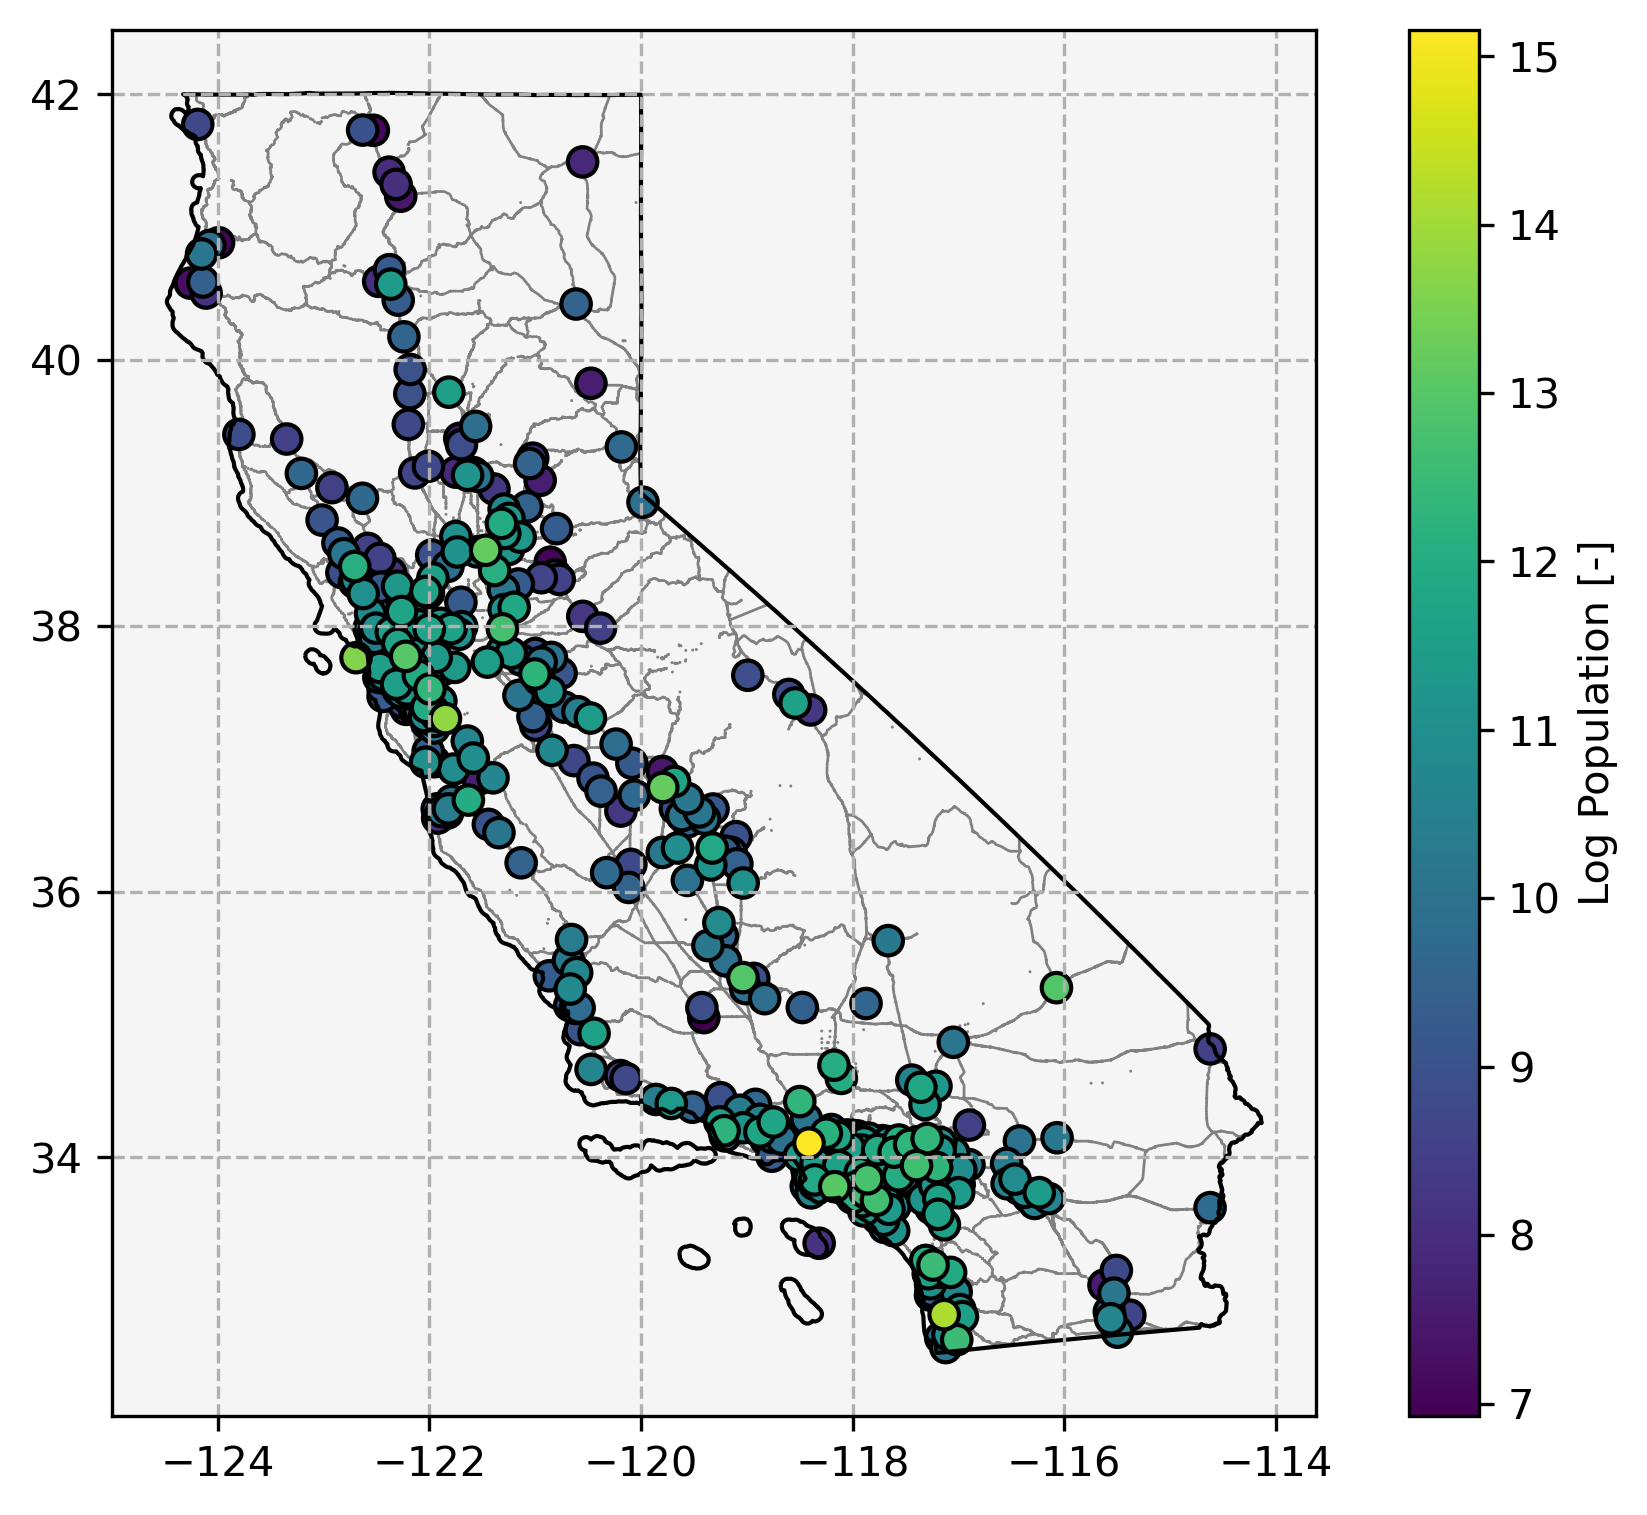
\includegraphics[width = \linewidth]{figs/california_incorporated_places.png}
	\caption{Natural logarithm of population for Incorporated Places in California}
	\label{fig:california_incorporated_places}
\end{figure}

Many of the most heavily populated Places are adjacent with each other or nearly so. The bulk of traffic between these will be local and routine. For the benefit of clarity and brevity these can be merged into super-Places. This is accomplished by the computation of maximally modular communities. First the distances for all pairs are computed. Second an inverse proximity is computed as

\begin{equation}
	\Gamma_{i,j} = \exp{\left(\frac{\Phi_d(i,j)}{\epsilon}\right)}
\end{equation}

where $\epsilon$ is a characteristic distance set at 10 km in this case. Solving for maximally modular communities, centroids of the 34 resulting communities are shown in Figure \ref{fig:california_incorporated_communities}.

\begin{figure}[H]
	\centering
	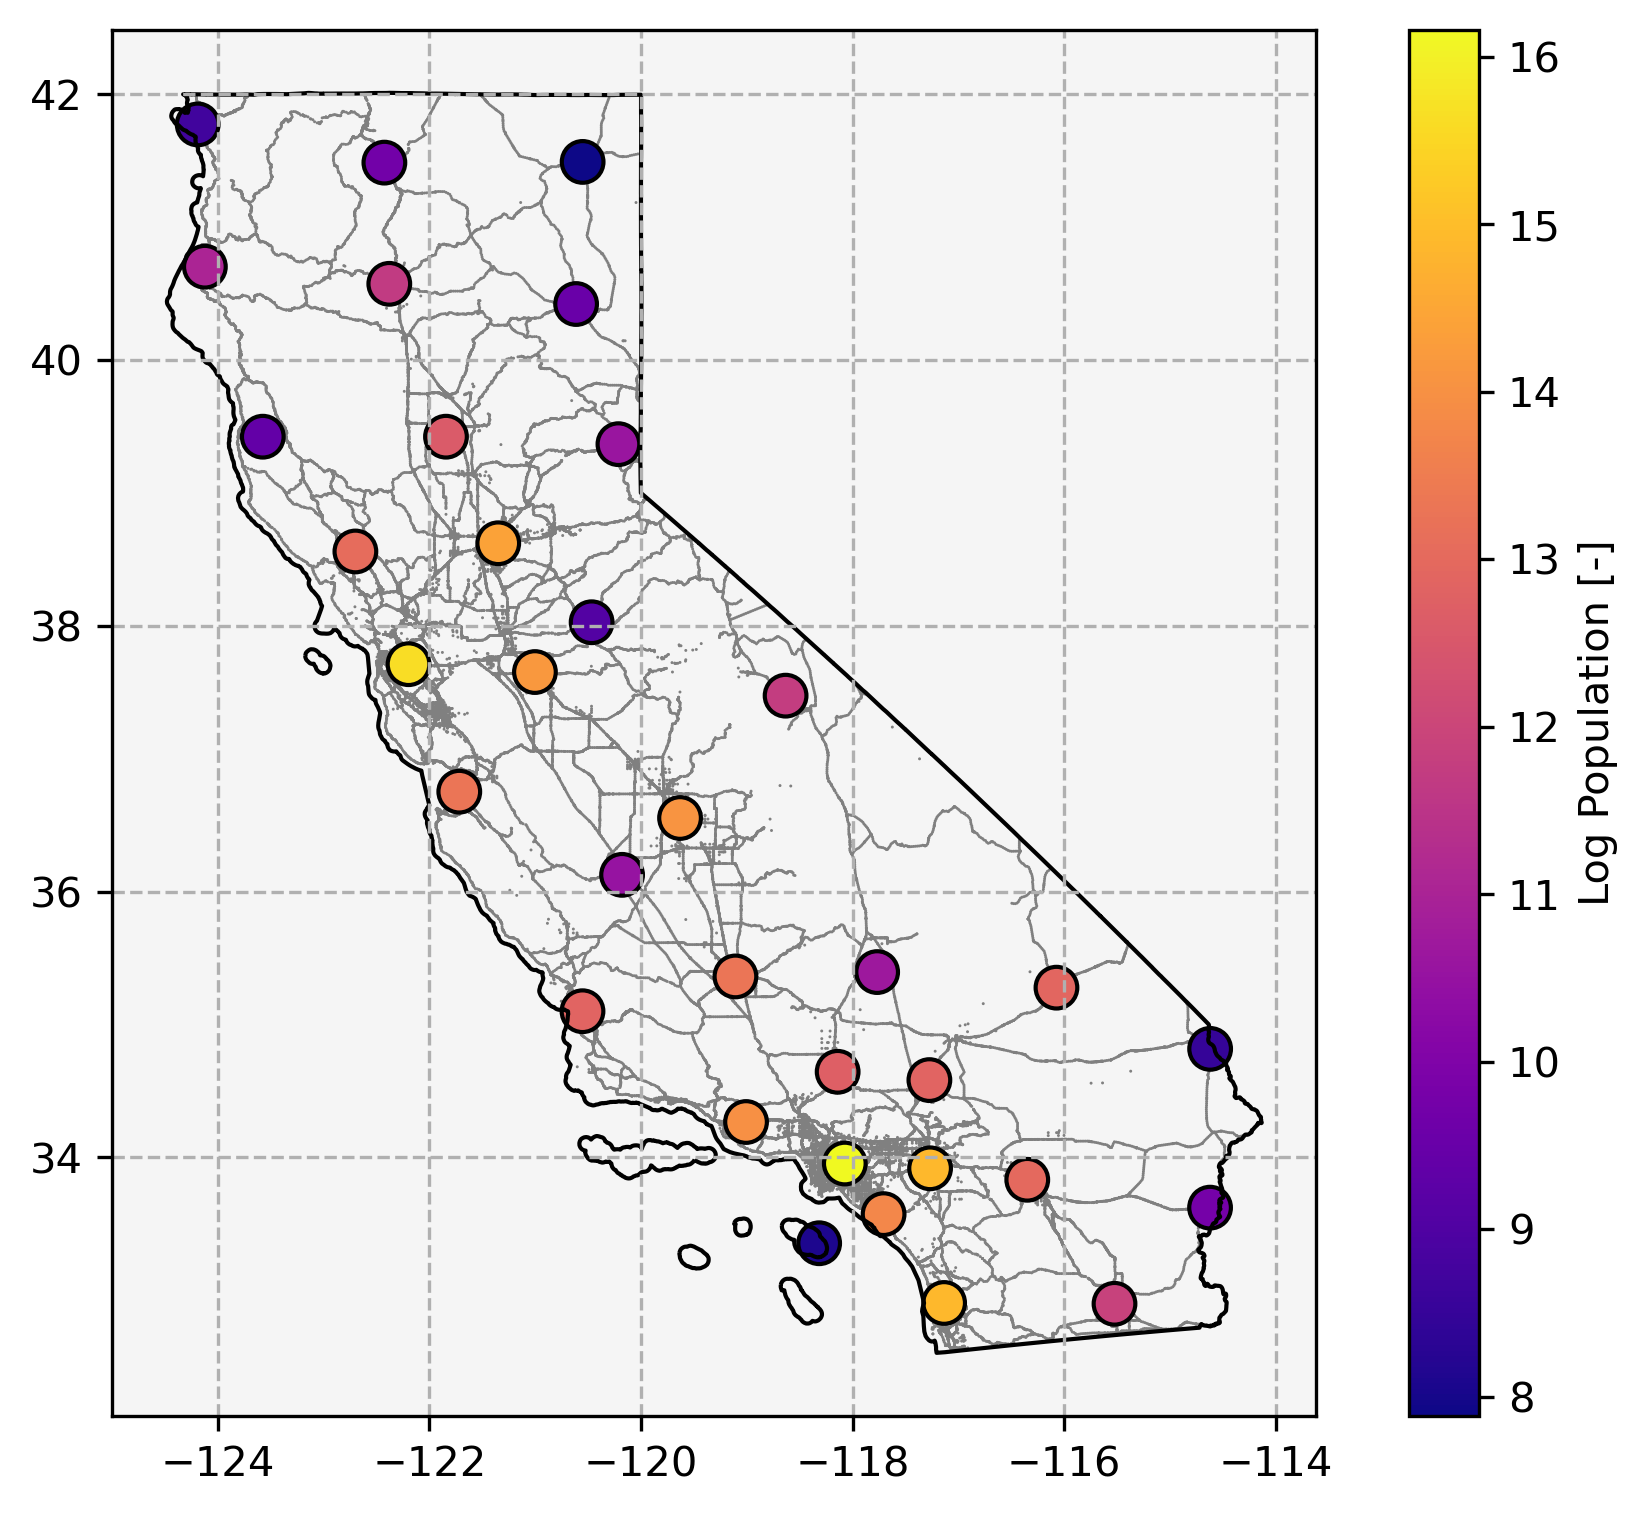
\includegraphics[width = \linewidth]{figs/california_incorporated_communities.png}
	\caption{Natural logarithm  of population for Incorporated Place Communities in California}
	\label{fig:california_incorporated_communities}
\end{figure}

Finally, for the purposes of analysis, points representing departure locations for Phoenix AZ, Las Vegas NV, Reno NV, and Portland/Eugene OR are added to the fringes of the map to represent the associated travel demand.

For long trips, \glspl{bev} will rely on DC charging stations. The locations of all DC charging stations in California are available from AFDC \cite{afdc_2023}. In may 2024 \gls{afdc} listed 2,149 active stations with at least 1 DC charger. This number is somewhat misleading as certain networks report each charger as an individual station even if within line-of-sight of one-another. After merging all stations of the same network which are within 100 meters direct distance of each other the number of stations becomes 1,689. California's DC charging stations include proprietary (vehicle \gls{oem} owned and operated) stations such as Tesla Superchargers and the Rivian Adventure network as well as non-proprietary stations such as those operated by ChargePoint, Electrify America, eVgo, and others. The selected locations and DC charging stations are mapped in Figure \ref{fig:california_stations}.

\end{multicols}

\begin{figure}[H]
\begin{subfigure}{\linewidth/3}
	\centering
	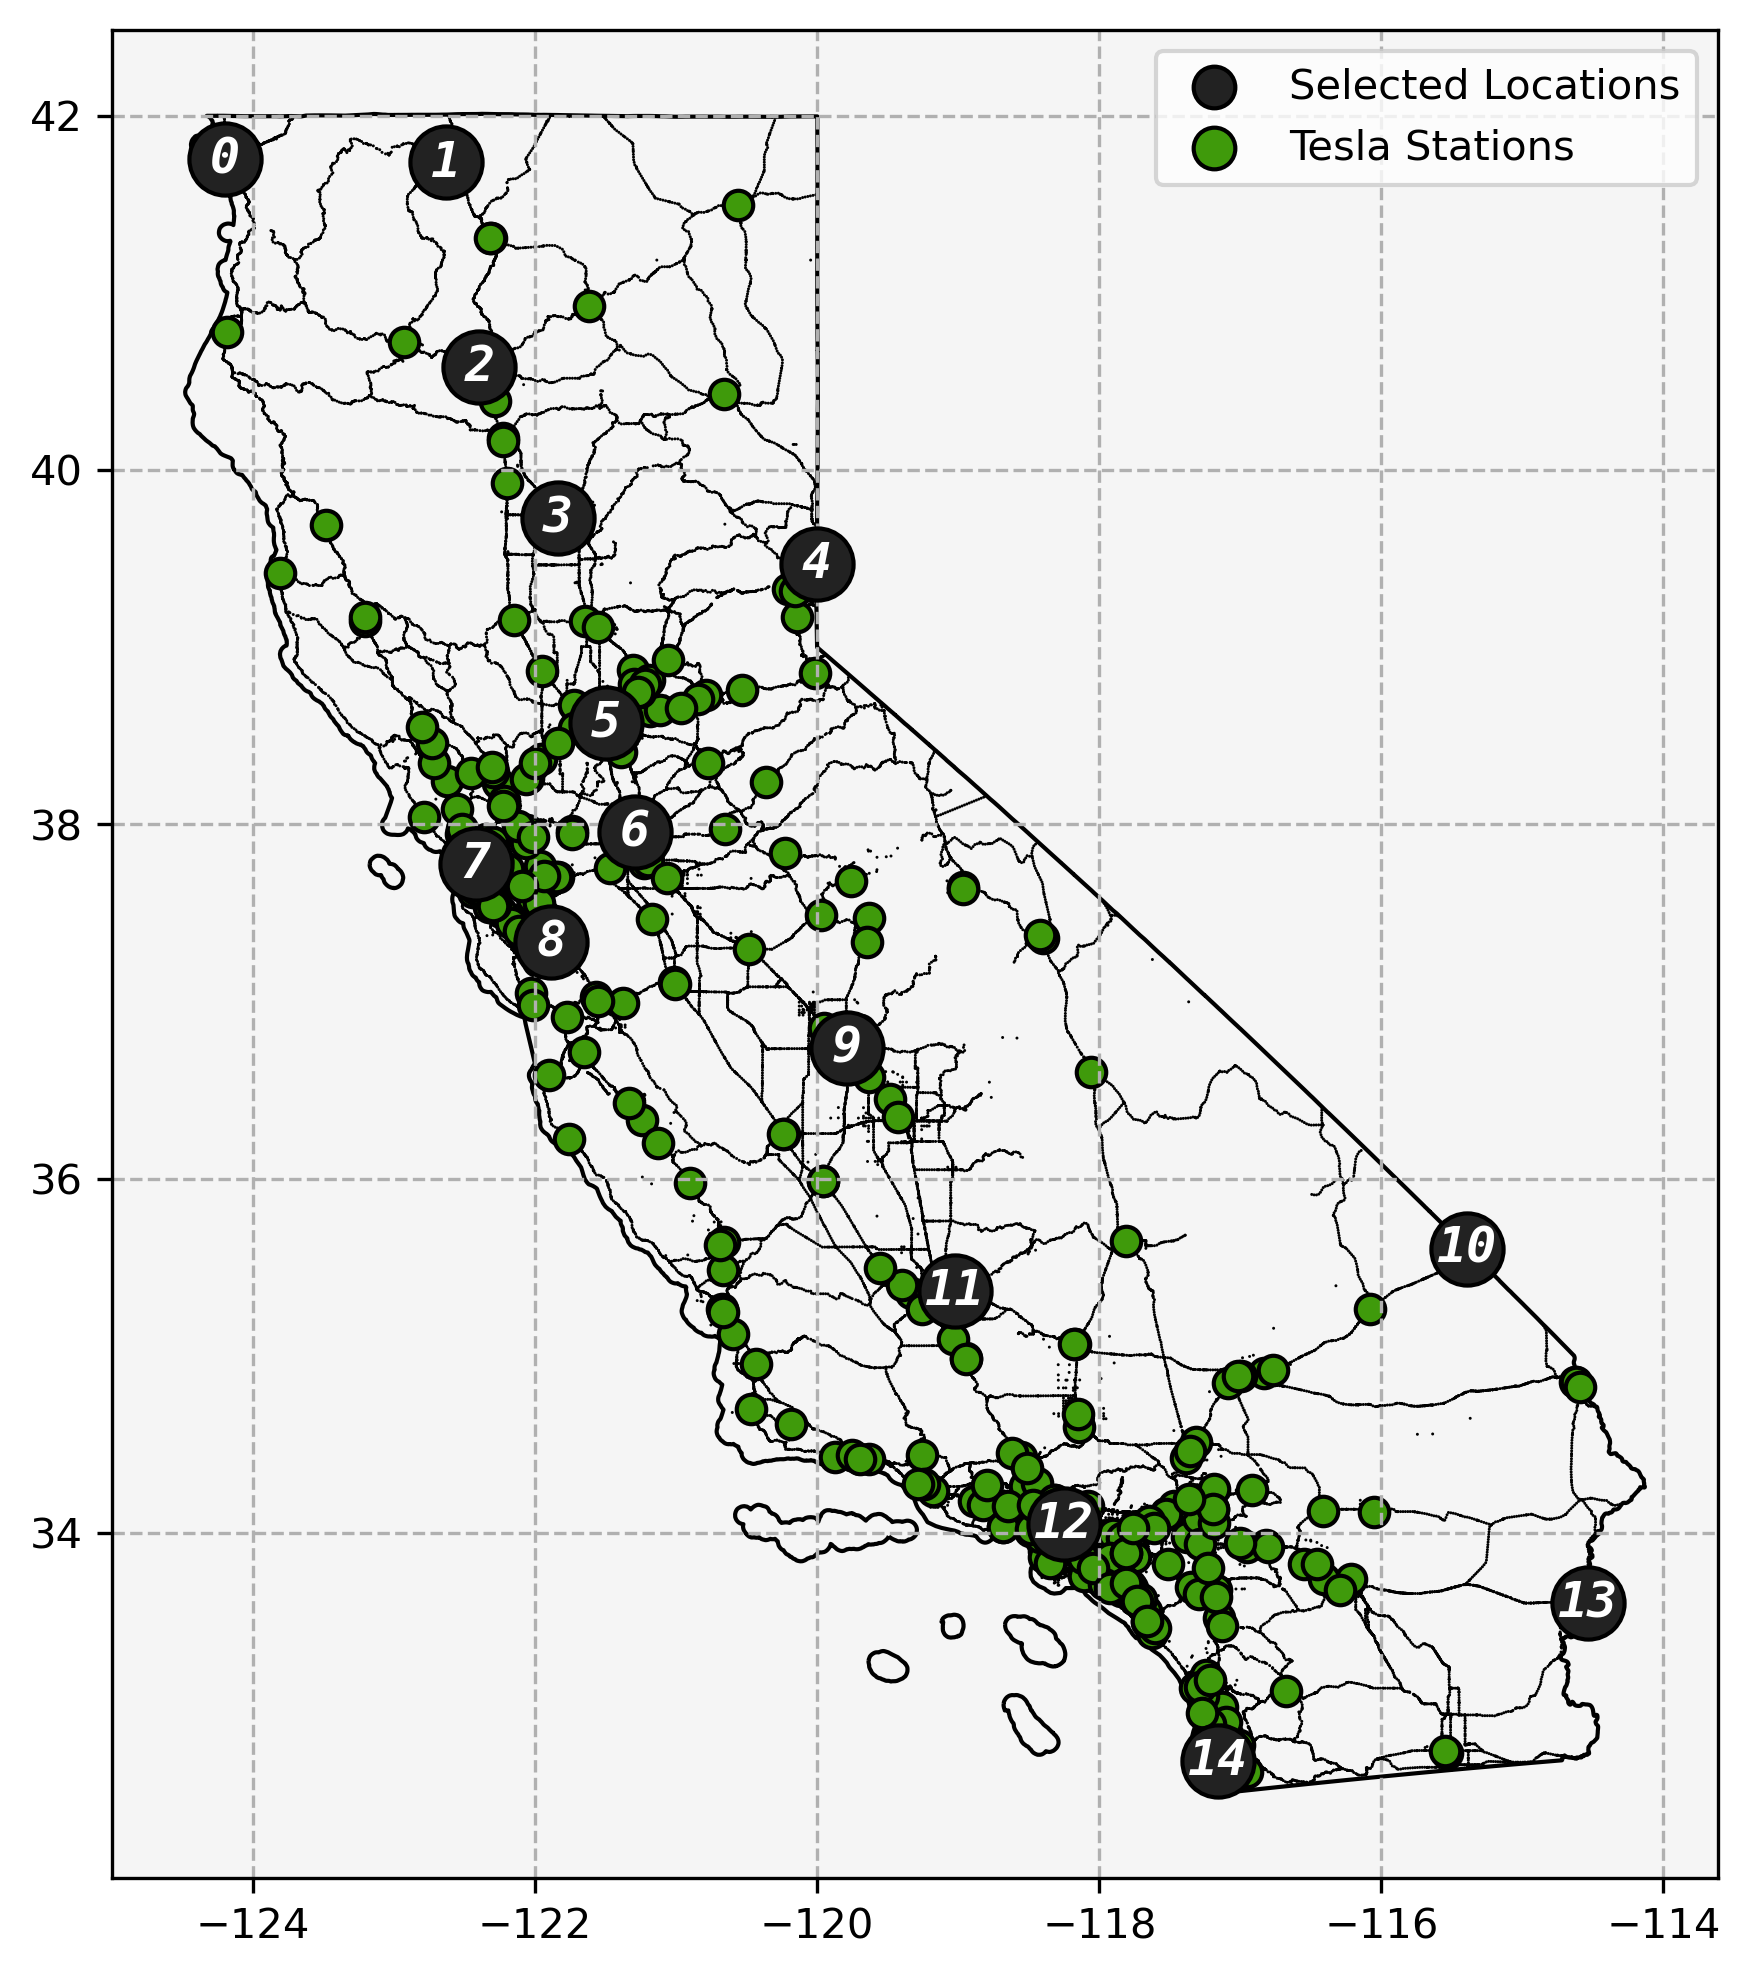
\includegraphics[width = \linewidth]{figs/California_SNG_T.png}
	\caption{Tesla Stations}
\end{subfigure}%
\begin{subfigure}{\linewidth/3}
	\centering
	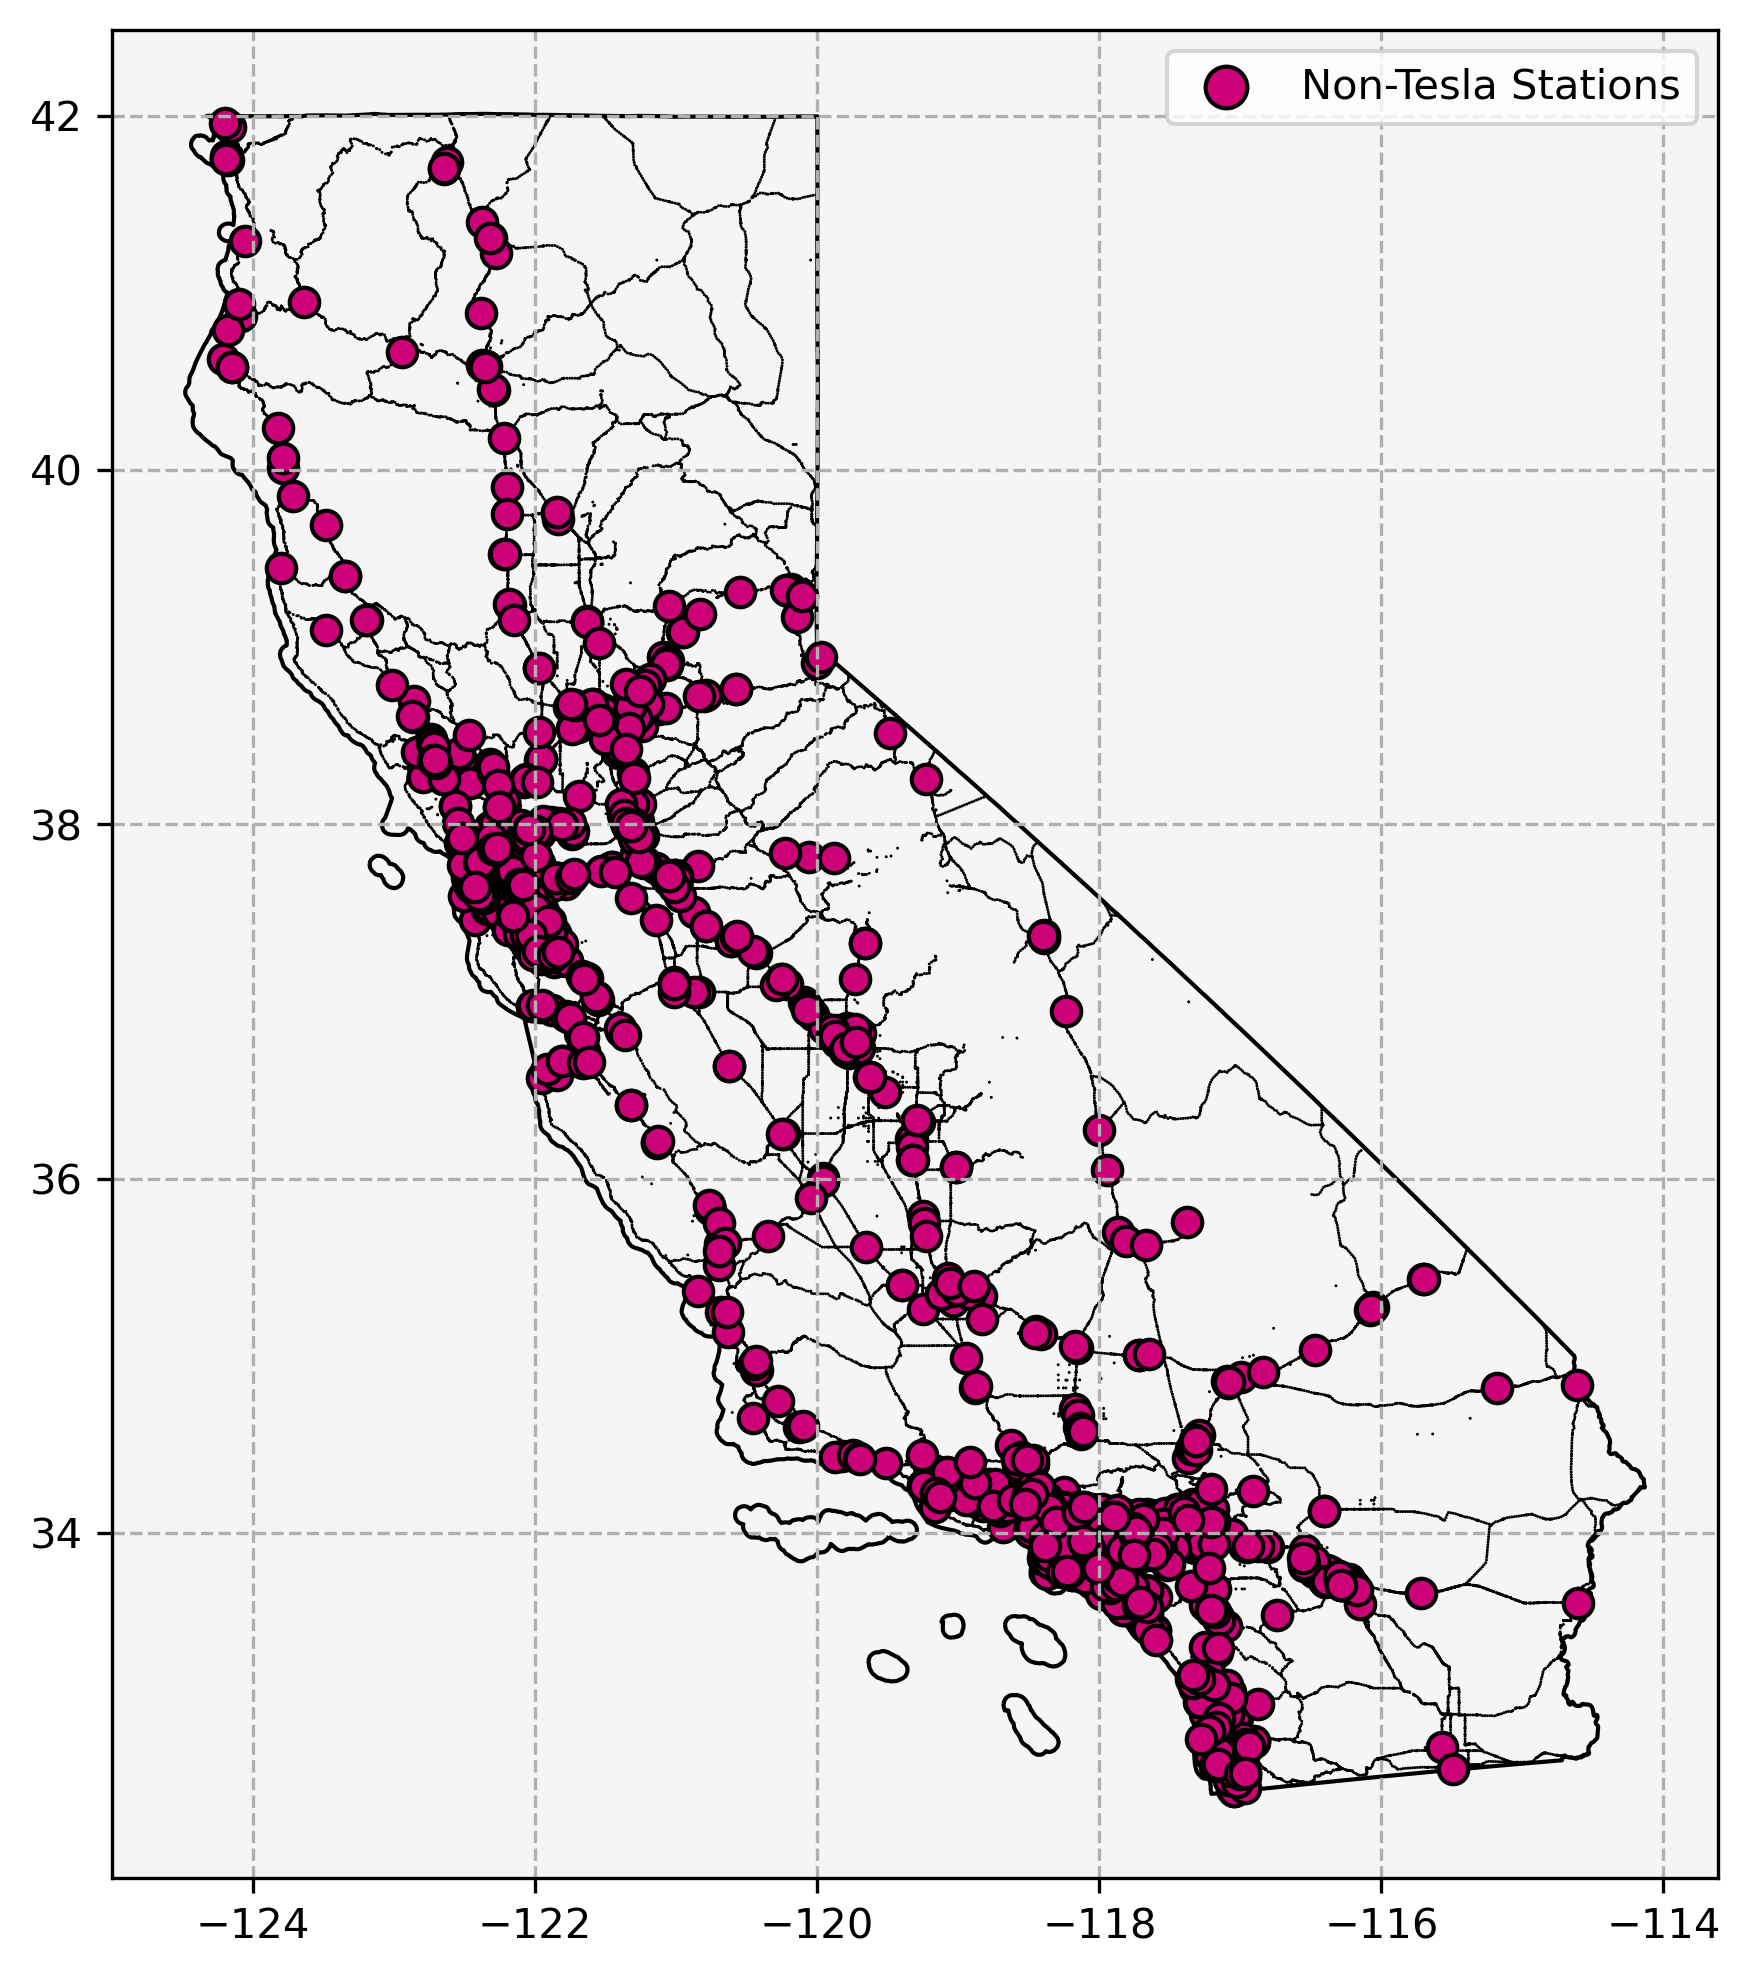
\includegraphics[width = \linewidth]{figs/California_SNG_NT.png}
	\caption{Non-Tesla Stations}
\end{subfigure}
\begin{subfigure}{\linewidth/3}
	\centering
	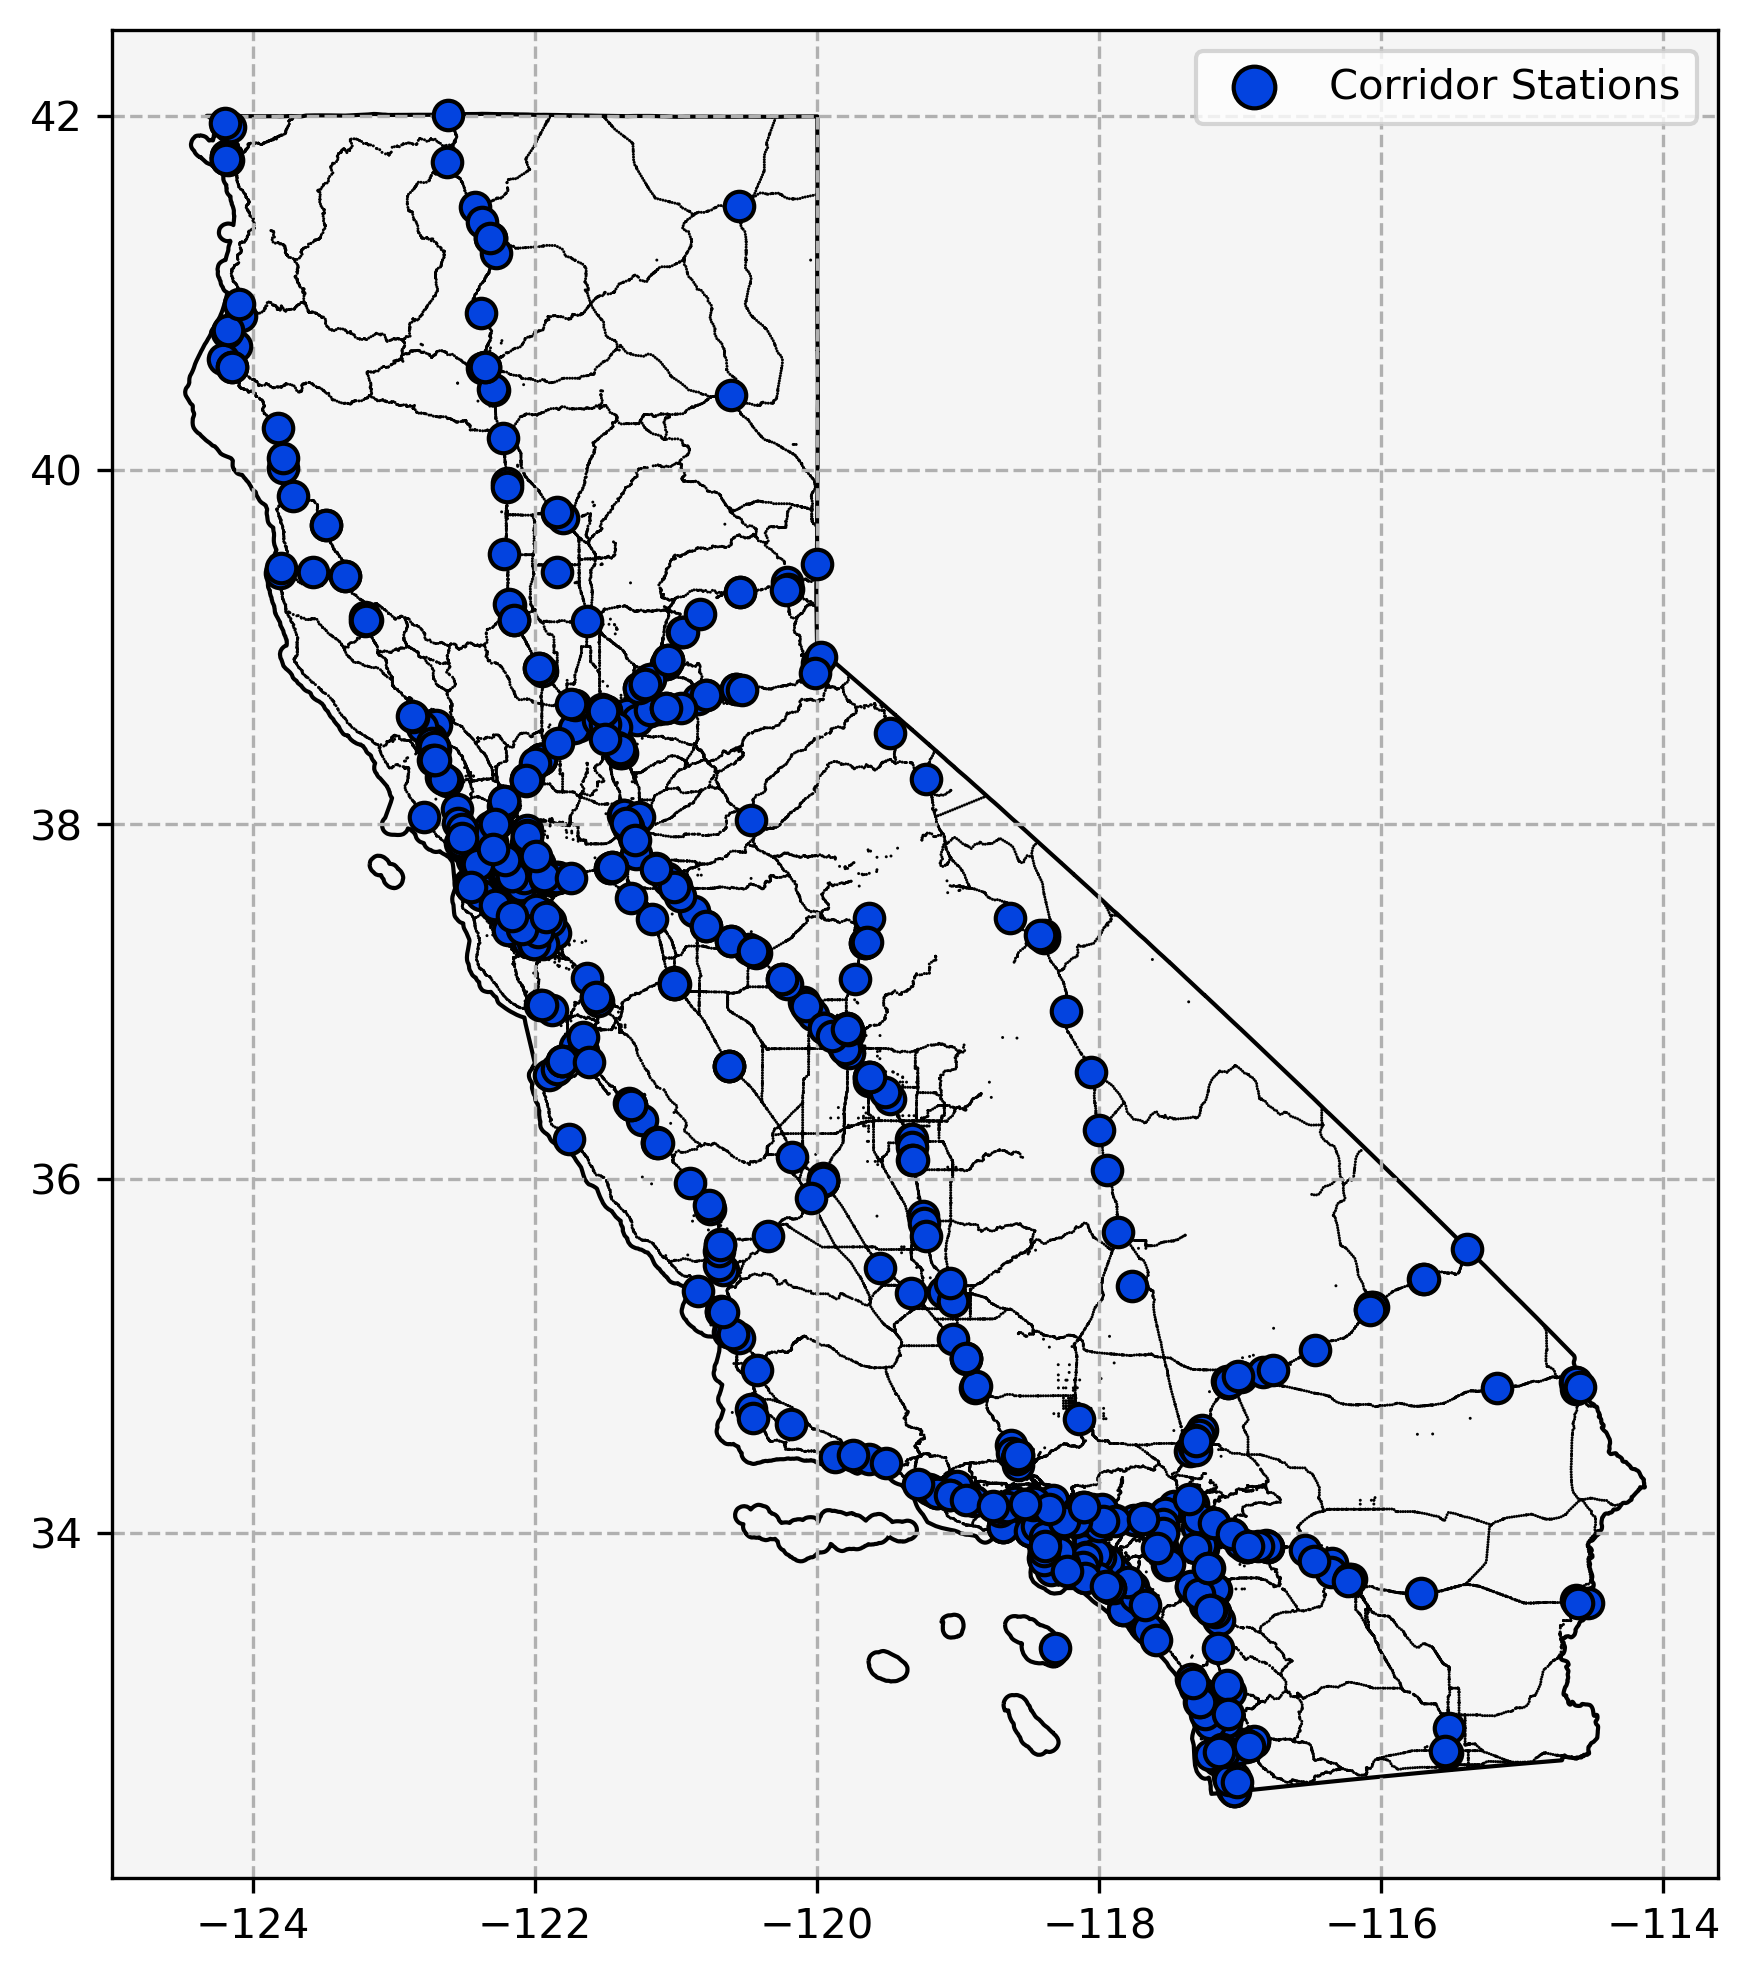
\includegraphics[width = \linewidth]{figs/California_SNG_Corridor.png}
	\caption{Corridor Stations}
\end{subfigure}
\caption{California DC charging stations from \gls{afdc} (May 2024)}
\label{fig:california_stations}
\end{figure}

\begin{multicols}{2}

There are 419 Tesla and 16 Rivian DC charging stations in the state as compared to 1,254 non-proprietary DC charging stations. In practice, many of these stations will be of little use for long distance travel being located far away from primary and secondary roads. Considering only those stations within 1 km of a highway as "corridor" chargers, there are a total of 500 corridor DC charging stations. Of the corridor stations, 156 are Tesla stations, 7 are Rivian stations, and 344 are non-Proprietary stations.

The non-Tesla networks overwhelmingly use CCS or combination CCS/ChaDeMo chargers which reflect the ports on the overwhelming number of non-Tesla \glspl{bev}. By contrast, Tesla chargers and vehicles use the NACS standard. The Tesla and non-Tesla systems are historically separate but increasingly interoperable with the aid of adapters. Tesla drivers use Tesla DC chargers almost exclusively \cite{Visaria_2022}. The Rivian Adventure network is technically interoperable with other J1772 vehicles but is set aside for the exclusive use of Rivian vehicles. The purpose of the Rivian Adventure network serves to allow for Rivian vehicles to charge in remote locations and is not intended to be relied upon exclusively.

The difference between the Tesla DC charging network and the non-Tesla networks extends from function to form. Built out as an investment to entice sales of Tesla vehicles and, until recently, exclusive to them, the Tesla network is technically superior with high maximum charging rates and more greater port usability rates \cite{Rempel_2023, Kozumplik_2022}. The Tesla network is mainly composed of high redundancy stations. Non-proprietary networks have, so far, been utilization and subsidy driven \cite{Gamage_2023} and are widely distributed with low redundancy stations. A stark contrast is seen when examining the ratios of chargers to stations. In California there are 403 Tesla DC charging stations with a total of 7,101 DC chargers for an average of 16.9 chargers per station. Among non-proprietary networks there are a total of 1,254 stations with 4,129 chargers for an average of 3.3 per station. Redundancies for Tesla and non-proprietary networks are shown in Figure \ref{fig:network_histograms}. 


\begin{figure}[H]
	\centering
	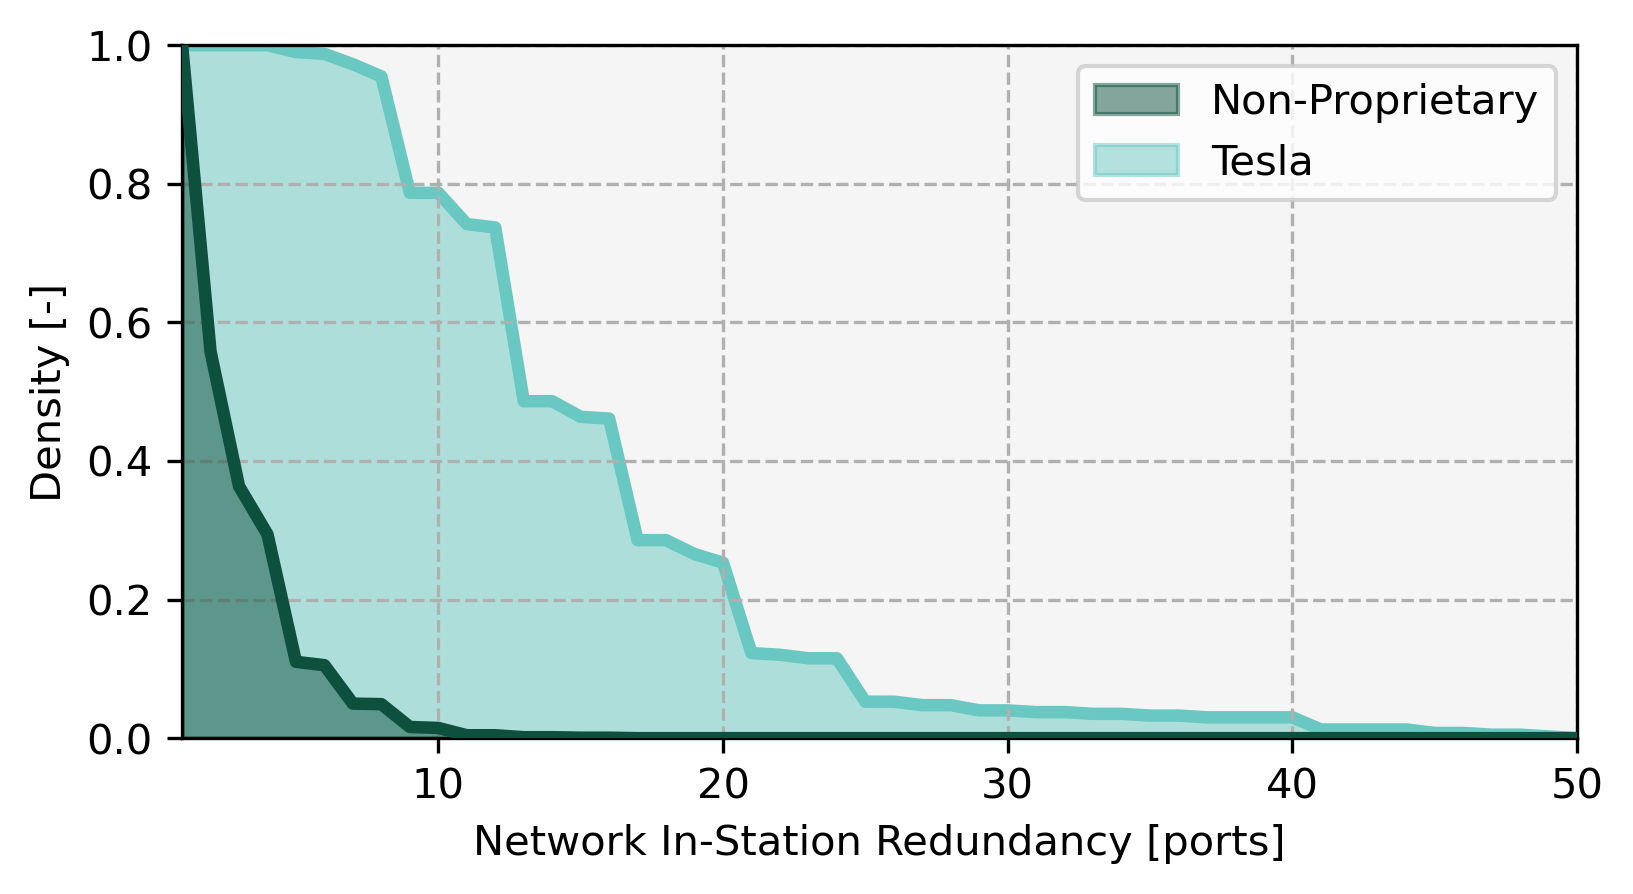
\includegraphics[width = \linewidth]{figs/California_RIS_Hist.png}
	\caption{Survival functions for in-station redundancy for Tesla and other DC charger networks in California}
	\label{fig:network_histograms}
\end{figure}

The Tesla DC charging network develops redundancy primarily in-station where the non-proprietary networks develop redundancy primarily between stations. Non-Tesla chargers are also more likely to be sighted in urban areas suggesting a desire to capture local as well as corridor travel demand. Tesla stations are more often sighted along travel corridors suggesting a focus on enabling long distance travel. In more remote parts of California the proprietary networks nearly match the non-proprietary networks in station numbers. In-station redundancies for DC charging networks in California can be found in Figures \ref{fig:ris_top_networks} and \ref{fig:ris_top_networks_corridor} in the Appendix. Summary statistics for DC charging networks in California can be found in Tables \ref{tab:summary_statistics_afdc} and \ref{tab:summary_statistics_afdc_corridor} in the appendix.

California \glspl{icev} utilize a third and completely separate network of supply stations. There are estimated to be over 8,000 gasoline stations in California \cite{CEC_2022} and these are widely and proportionally distributed. Because no public database for the locations of gasoline stations in the state exists, and due to their ubiquity it is assumed in this study that \gls{icev} driver optimal paths will not be effected by fueling station availability. For this reason, \glspl{icev} are, herein, assumed to take the "direct" path between cities where \glspl{bev} need to find optimal paths on their \glspl{sng}.

\subsection*{Experiment}

In order to understand the effects of vehicular, infrastructural, and behavioral parameters on road-trip accessibility an experiment was carried out on randomly generated combinations. As a baseline, three \glspl{icev} were also modeled. These \glspl{icev} represent different levels of efficiency present in the \gls{icev} fleet. \gls{ess} capacity numbers are pulled from manufacturer websites and energy consumption rates are computed from EPA highway fuel economy ratings \cite{DOE_EPA_2024}. Although substantially less efficient than equivalent \glspl{bev} the comparatively high specific energy of liquid petroleum allows for \glspl{icev} to have higher maximum ranges. \gls{icev} supply infrastructure is modeled to dispense fuel at the normal US rate of 7 gallons per minute which is an equivalent energy supply rate of 14.15 MW. When refueling, the Prius. Golf, and Pacifica, add highway range at rates of 631, 462, and 282 km per minute respectively. The \gls{icev} models and corresponding Regional Impedance values are shown in Table \ref{tab:icev_models}.

\begin{table}[H]
	\centering
	\caption{\gls{icev} models}
	\label{tab:icev_models}
	\begin{tabular}{|C{.45\linewidth}|C{.3\linewidth}|C{.25\linewidth}|}
		\hline Vehicle Model & Parameter & Value \\
		\cline{1-3} & \gls{ess} Capacity & 381 [kWh] \\
		\cline{2-3} & Energy Consumption & 1,346 [kJ/km] \\
		\cline{2-3} 2024 Toyota Prius & Full-Tank Range & 1,018 [km] \\
		\cline{2-3} & California Regional Impedance & 4.131 [hours] \\
		\cline{1-3} & \gls{ess} Capacity & 445 [kWh] \\
		\cline{2-3} & Energy Consumption & 1,839 [kJ/km] \\
		\cline{2-3} 2024 Volkswagen Golf & Full-Tank Range & 871 [km] \\
		\cline{2-3} & California Regional Impedance & 4.151 [hours] \\
		\cline{1-3} & \gls{ess} Capacity & 640 [kWh] \\
		\cline{2-3} & Energy Consumption & 3,015 [kJ/kM] \\
		\cline{2-3} 2024 Chrysler Pacifica & Full-Tank Range & 764 [km] \\
		\cline{2-3} & California Regional Impedance & 4.161 [hours] \\
		\hline
	\end{tabular}
\end{table}

Regional Impedance for \glspl{icev} was computed under the assumption of petroleum supply infrastructure ubiquity. As such, \glspl{icev} were given the "direct" path between locations with stop times added where additional range was needed. For each necessary stop, time was added for refueling to full as well as 10 minutes to divert from the road and handle the transaction prior to refueling. Additionally, drivers of the \glspl{icev} were assumed to keep a 10\% buffer of remaining range. The \glspl{icev} each had similar road-trip accessibility scores of roughly 5.5 hours. The longest arc considered in Crescent City (Location 0) to Phoenix - State Line (Location 13) which is roughly 1,530 km just exceeding double the usable range of the Pacifica. The Prius, Golf, and Pacifica required averages of 0.43, 0.31, and 0.19 supply stops per route respectively.

500 random scenarios were generated by uniform random sampling of the parameters listed in Table \ref{tab:experimental_parameters} and run on three \glspl{sng} as described in \ref{tab:experimental_sngs}. All randomly sampled \glspl{bev} in this study are assumed to have an energy consumption rate of 608 kJ/km this being the EPA energy consumption rate of a Tesla Model 3 in highway operation \cite{DOE_EPA_2024}. Highway operation is assumed herein due to the focus on long trips. Thus \gls{bev} full-charge ranges will be between 237 and 711 km. Vehicles are assumed to fast charge only up to 80\% \gls{soc} in order to remain in the constant current range. When charging, sampled \glspl{bev} add highway range at a rate between 4.9 and 19.7 km per minute. Risk attitude was modeled as in \eqref{eq:superquantile} with the range centered around the mean parameter $\overline{p}$ where $p_0 = \overline{p} - .1$ and $p_1 = \overline{p} + .1$. 

\begin{table}[H]
	\centering
	\caption{Parameters and ranges for experiment.}
	\label{tab:experimental_parameters}
	\begin{tabular}{|C{\linewidth/2}|C{\linewidth/2}|}
		\hline Parameter & Range \\
		\hline \gls{ess} Capacity & [40 kWh, 120 kWh] \\
		\hline \gls{ess} Max Charge Rate & [50 kW, 200 kW] \\
		\hline Driver Risk-Attitude Mean & [.1, .9] \\
		\hline \gls{evse} Reliability & [.5, 1] \\
		%		\hline Station Arrival Ratio Mean & [1, 3] \\
		\hline
	\end{tabular}
\end{table}

\begin{table}[H]
	\centering
	\caption{\glspl{sng} used in experiment.}
	\label{tab:experimental_sngs}
	\begin{tabular}{|C{\linewidth/3}|C{\linewidth*2/3}|}
		\hline Label & Networks Included \\
		\hline Combined & All stations \\
		\hline Tesla & Only Tesla stations \\
		\hline Non-Tesla & All non-Tesla stations \\
		\hline
	\end{tabular}
\end{table}

Outputs were processed to compute a population weighted Regional Impedance as in \eqref{eq:regional_impedance}. Impedance was selected as the metric of evaluation rather than accessibility as travel demand for each arc was the same for all cases. Linear regression was performed on the results of the random experiment. Using as output, the neutral expectation of road-trip accessibility for each of the 500 randomly sampled vehicles on each of the \glspl{sng}. Significant parameters from the regression are shown in Figure \ref{fig:significant_parameters}.

\begin{figure}[H]
	\centering
	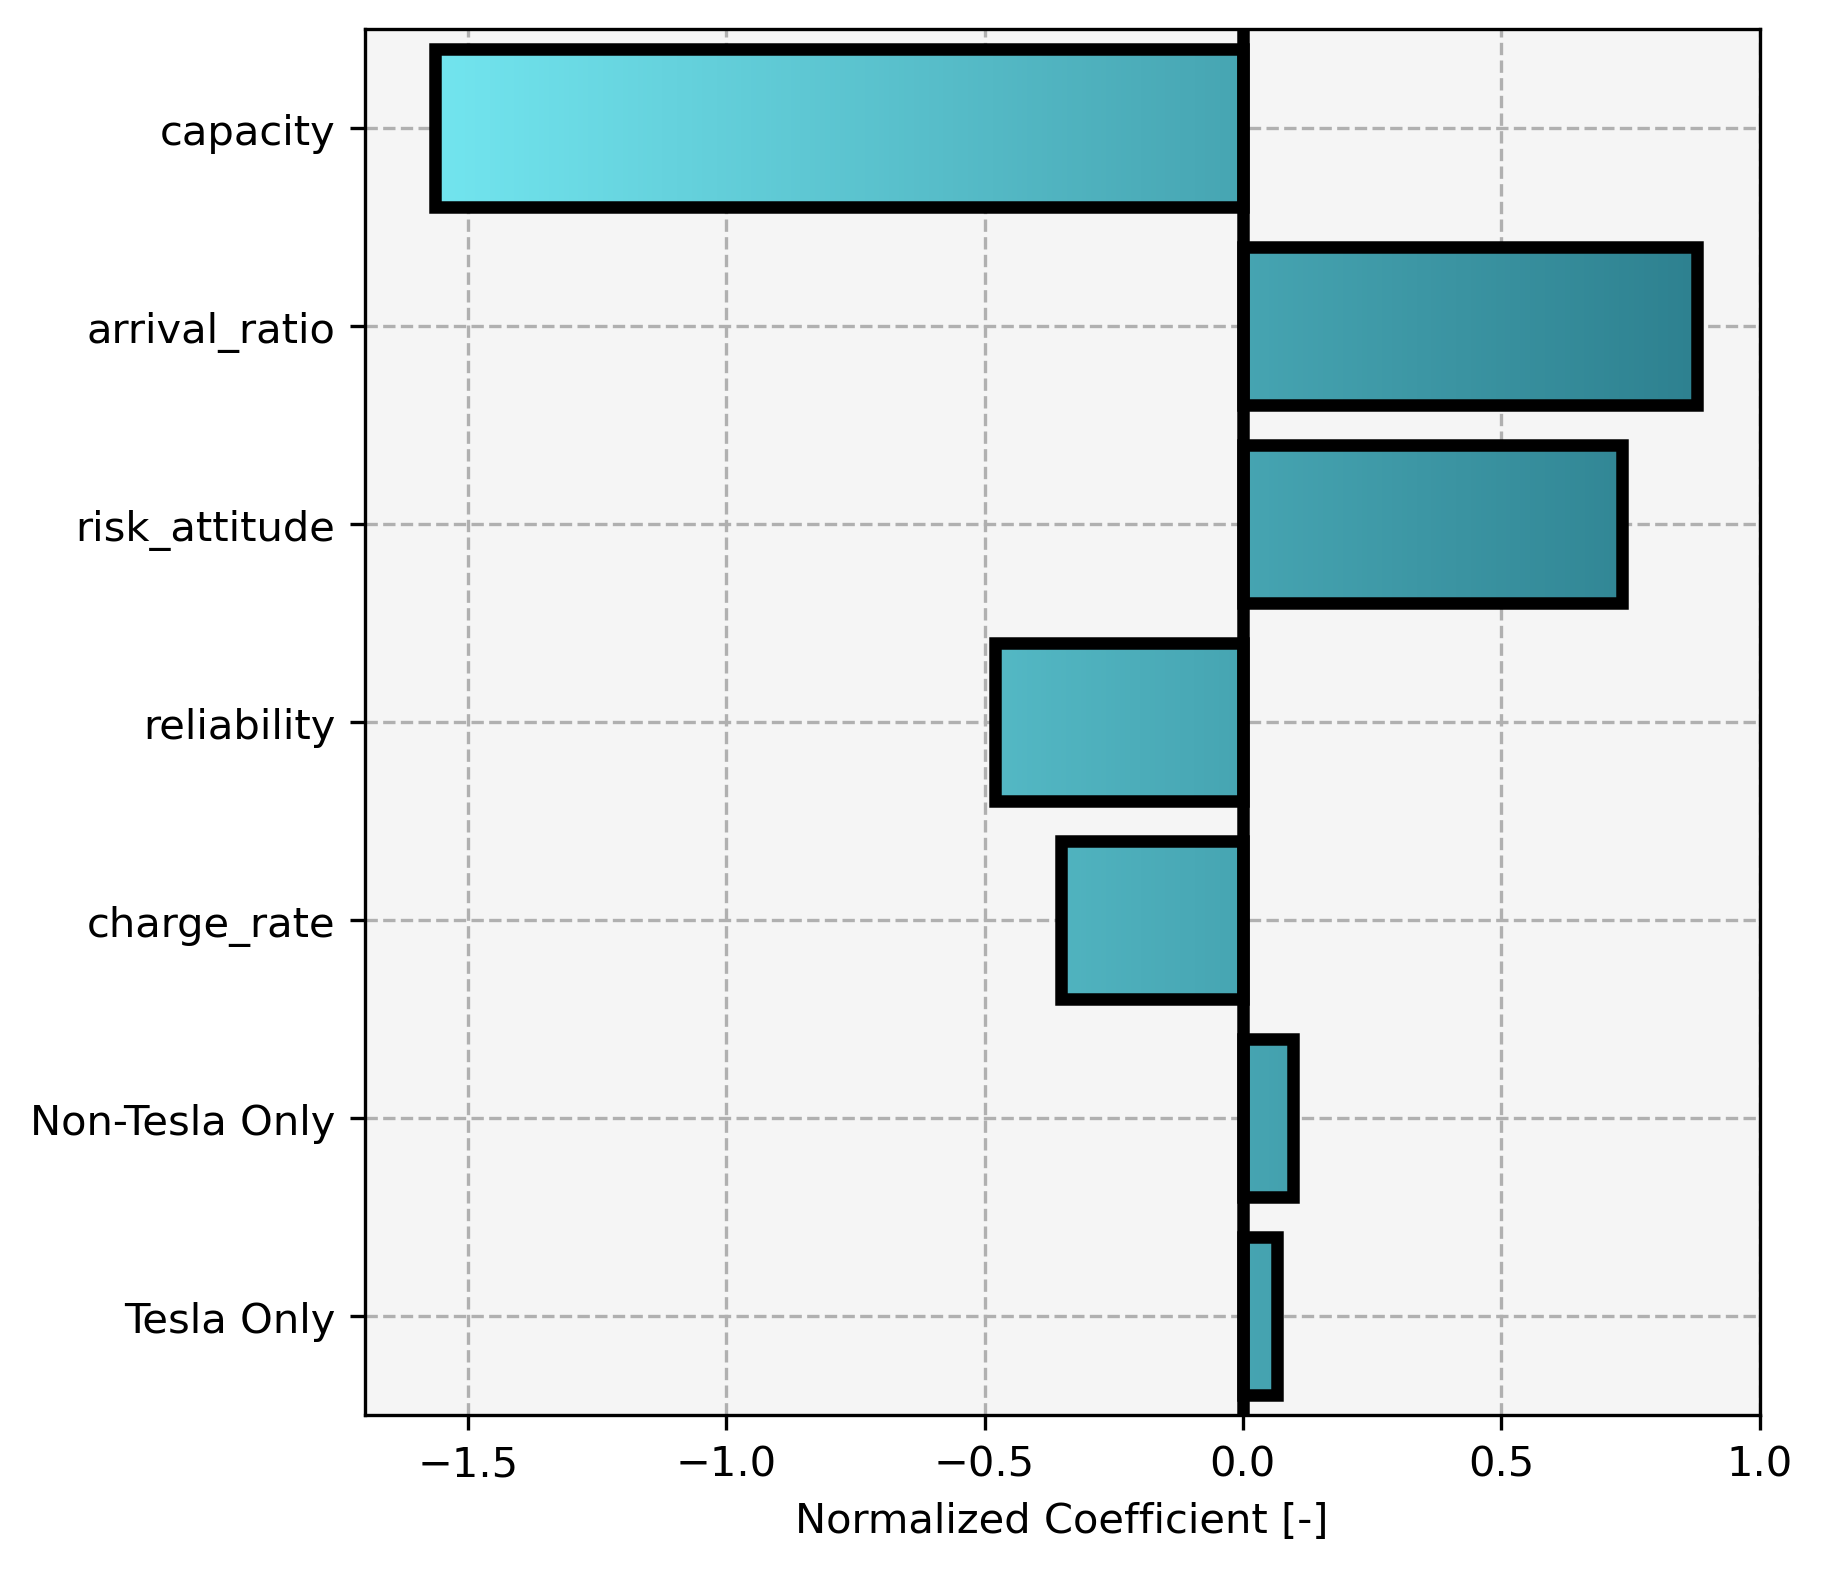
\includegraphics[width = \linewidth]{figs/significant_parameters.png}
	\caption{Coefficients for significant parameters from linear regression}
	\label{fig:significant_parameters}
\end{figure}

Regression details are provided in Tables \ref{tab:regression_anova} and \ref{tab:regression_coefficients} in the Appendix. The regression analysis shows that vehicular, infrastructural, and behavioral parameters have significant impacts on road-trip accessibility. The vehicular parameters of capacity and charge rate have the predictable effect of reducing expected travel times. Capacity being the more more important parameter is explicable as higher capacity vehicles offer the ability to stop less frequently. Saving an entire charging event can be very impactful in a region the size of California. Among the infrastructure parameters, higher reliability contributed to lower travel times where higher arrival ratios contributed to higher travel times. Both reliability and arrival ratio primarily effect queuing times as, even with 50\% equipment reliability, most stations have sufficient redundancy to guarantee at least one operational charger. The range of arrivals ratios considered goes from normal to swamped and long queues can be expected for high arrival ratios even at high redundancy stations. Risk attitude was also significant in determining outcomes as those drivers with more cautious risk attitudes will tend to maintain higher \gls{soc} and utilize more reliable and redundant routes. finally, access to the entire network is better than restriction to just part of it but being restricted to only Tesla stations should be slightly less damaging than access to only non-Tesla stations. Boxplots of expected travel times are shown in Figure \ref{fig:networks_boxplots}.

\begin{figure}[H]
	\centering
	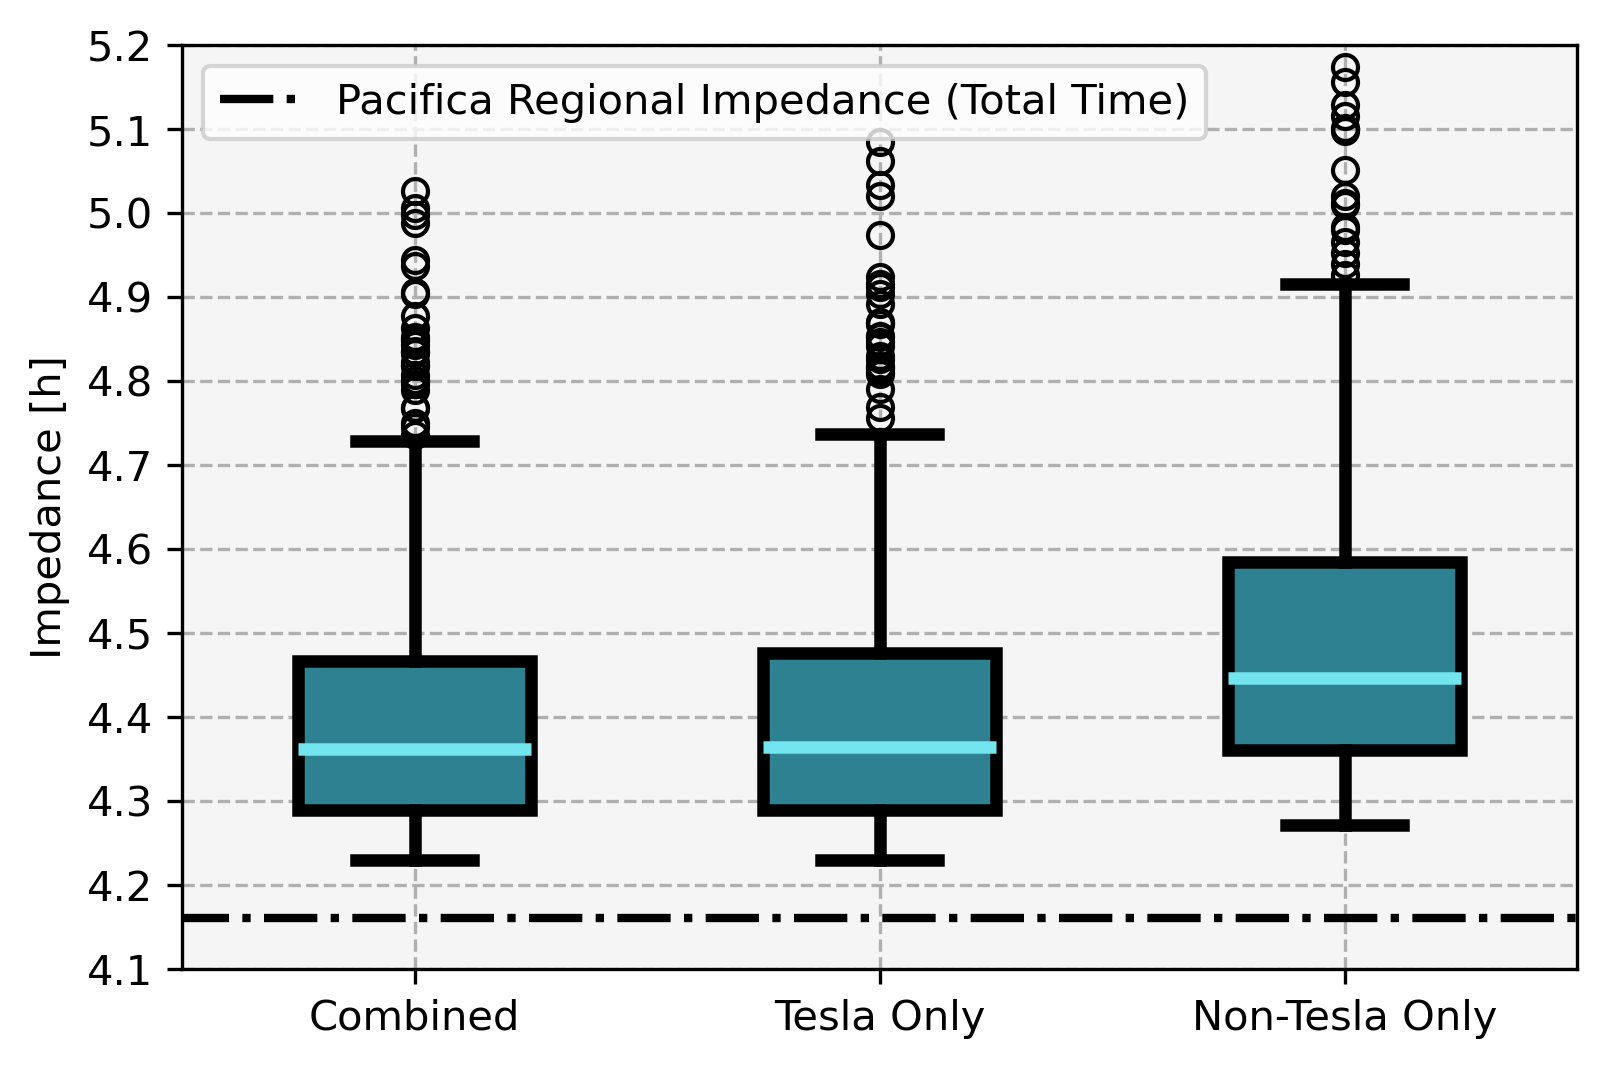
\includegraphics[width = \linewidth]{figs/Networks_Boxplots_Weighted_Impedance.png}
	\caption{Boxplots of experiment outputs by \gls{sng}}
	\label{fig:networks_boxplots}
\end{figure}

While the differences between the \glspl{bev} on the basis of \gls{sng} access are observed to be slight, the differences between the means of each and the worst of the \glspl{icev} is quite large. The difference is roughly 45 minutes much of which can be explained by the shorter ranges and longer supply times inherent to the \glspl{bev}. In the best of circumstances, \glspl{bev} can reach near parity with \glspl{icev}. However, \glspl{bev} impedance will, nearly always, be substantially higher than \gls{icev} impedance due to the necessity of charging events. Some will argue that this difference is unimportant as \gls{bev} drivers can charge their vehicles while stopping for meals or during other natural breaks. This logic has been used to show that \glspl{bev} may approach convenience parity with \glspl{icev} in reasonable circumstances \cite{Dixon_2020}. However, where such long breaks are optional for \gls{icev} drivers, they are mandatory for \gls{bev} drivers and must be taken at specific points throughout the trip to coincide with charging. This loss of optionality must be accounted an inconvenience even for drivers who accustomed to long breaks.

Most of the difference in impedance is due to charging and queuing times while only a small part is due to route alterations. Isolating the driving times by subtracting supply and setup times, the differences between \glspl{bev} and \glspl{icev} \glspl{sng} are substantially smaller than those in total trip time as shown in Figure \ref{fig:networks_boxplots_driving}. It should, however, be noted that there is a long tail on the driving time distributions due to the occasional need to take a significantly altered route to confidently reach a remote destination.

\begin{figure}[H]
	\centering
	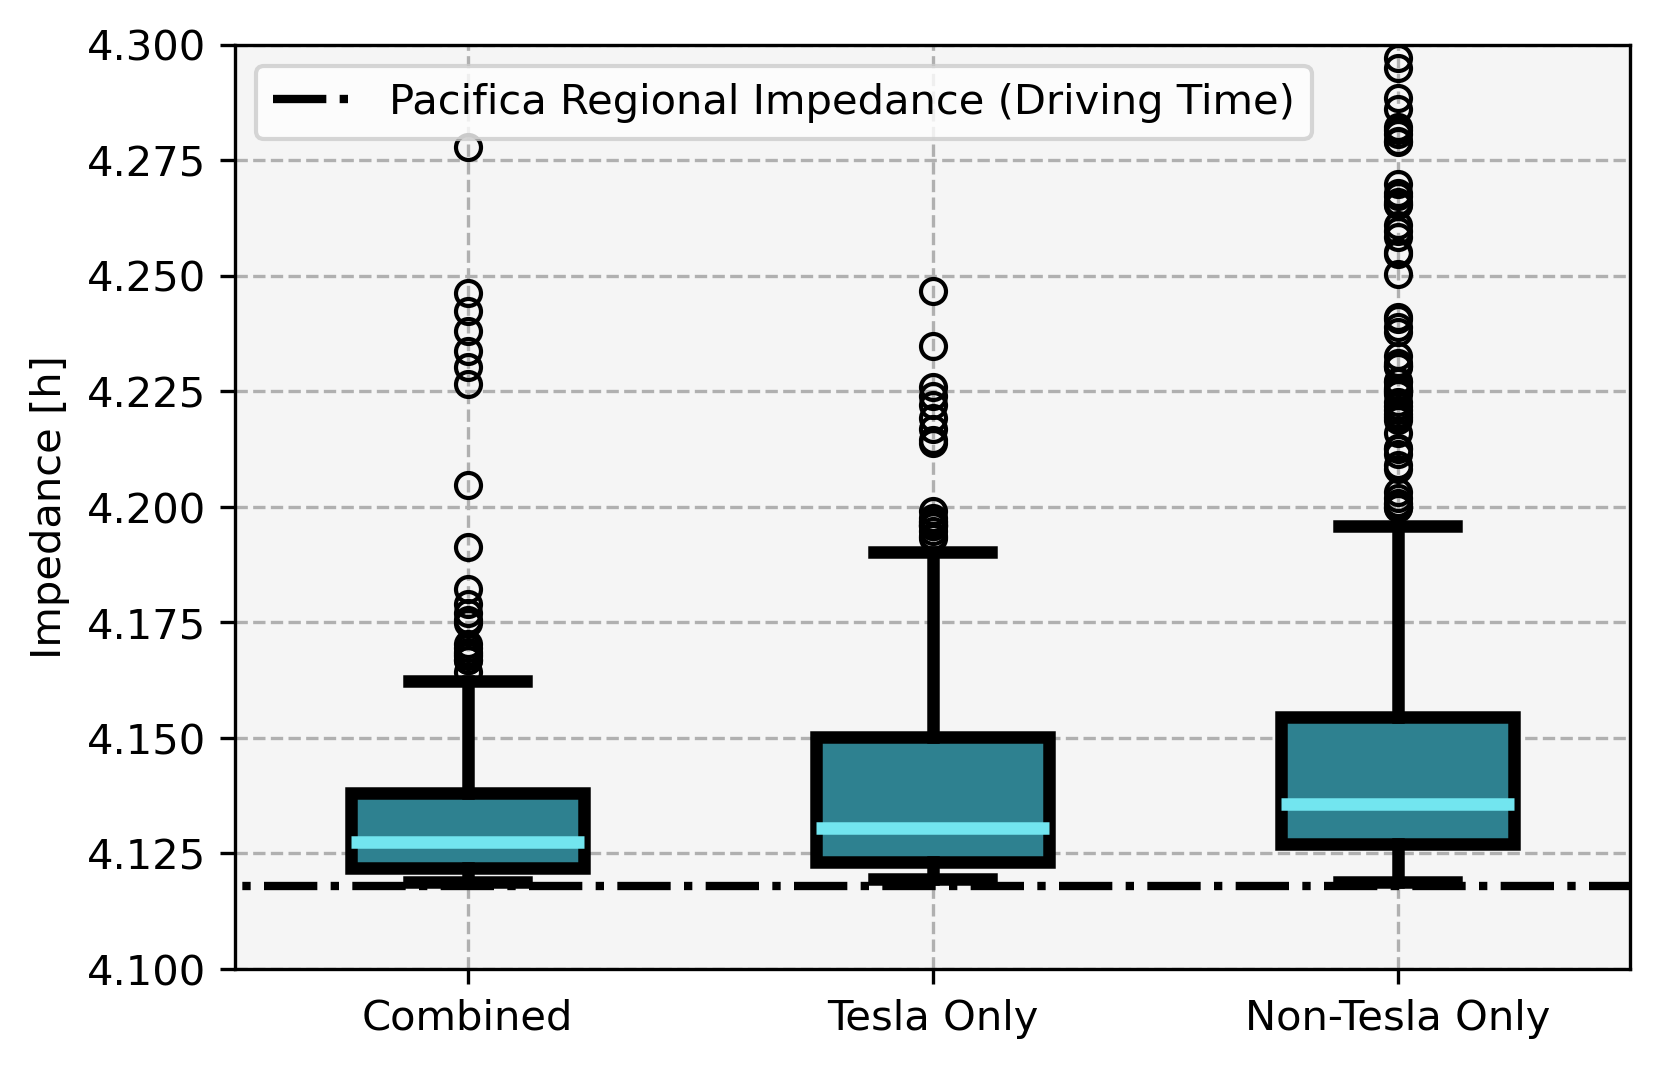
\includegraphics[width = \linewidth]{figs/Networks_Boxplots_Weighted_Impedance_Driving.png}
	\caption{Boxplots of experiment outputs by \gls{sng} (driving time only)}
	\label{fig:networks_boxplots_driving}
\end{figure}

Different parts of the state will have different experiences. Residents of large population centers which are proximate to other large population centers will expect to have lower travel needs than those in more remote areas. In general, the impedance disparities associated with different vehicular, infrastructural, and behavioral characteristics will also scale with impedance. As California is a large state with a diversity of land use and road infrastructure volume, there is a pronounced difference in Specific Regional Impedance as shown in Figure \ref{fig:networks_boxplots_locations}.

\end{multicols}

\begin{figure}[H]
\centering
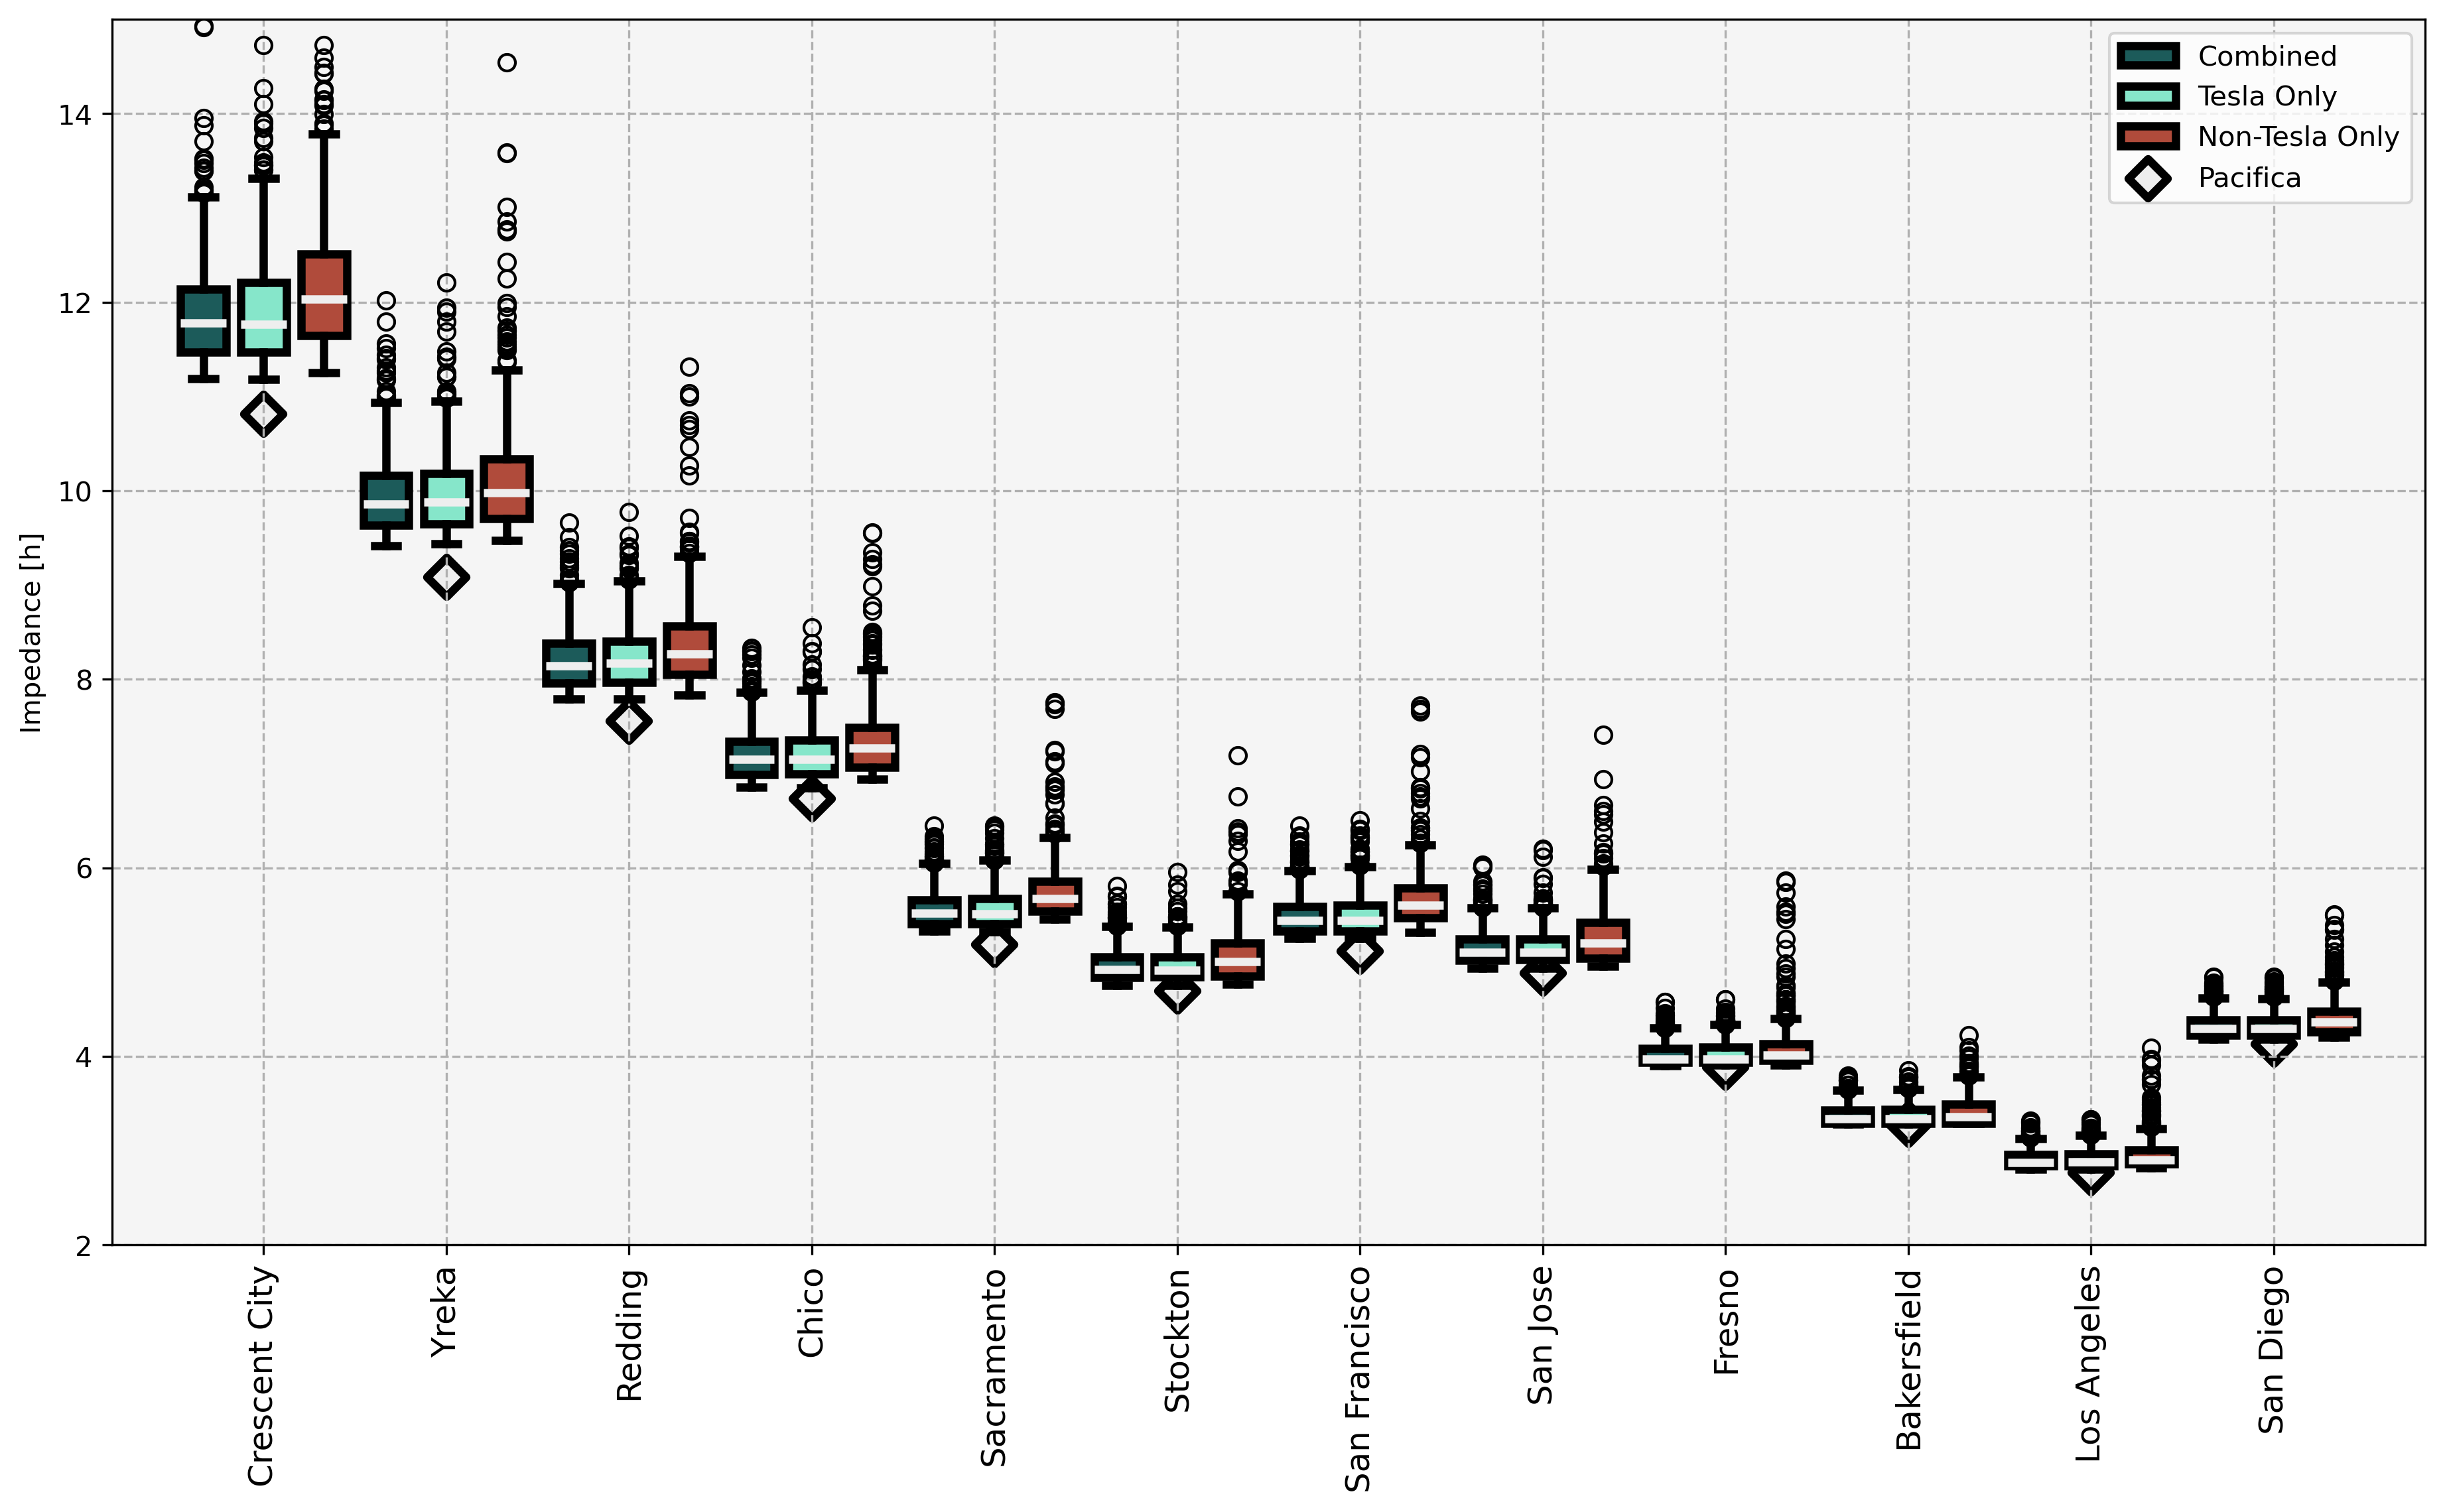
\includegraphics[width = \linewidth]{figs/Networks_Boxplots_Weighted_Specific_Impedance_2.png}
\caption{Boxplots of experiment outputs on combined \gls{sng} for each origin in California}
\label{fig:networks_boxplots_locations}
\end{figure}

\begin{multicols}{2}
	
\section*{Discussion}

The optimal routes generated in this study only selected corridor chargers. Some insight into the utility provided by each network can be gained by looking into utilization rates for networks and stations when using the combined \gls{sng}. Ratio of stations utilized at least once to total corridor stations in the combined \gls{sng} for each network is shown in Figure \ref{fig:utilization_rates}. Log of utilization (number of times utilized in random experiment) for corridor stations in the combined \gls{sng} is displayed in Figure \ref{fig:utilized_stations}.

\begin{figure}[H]
	\centering
	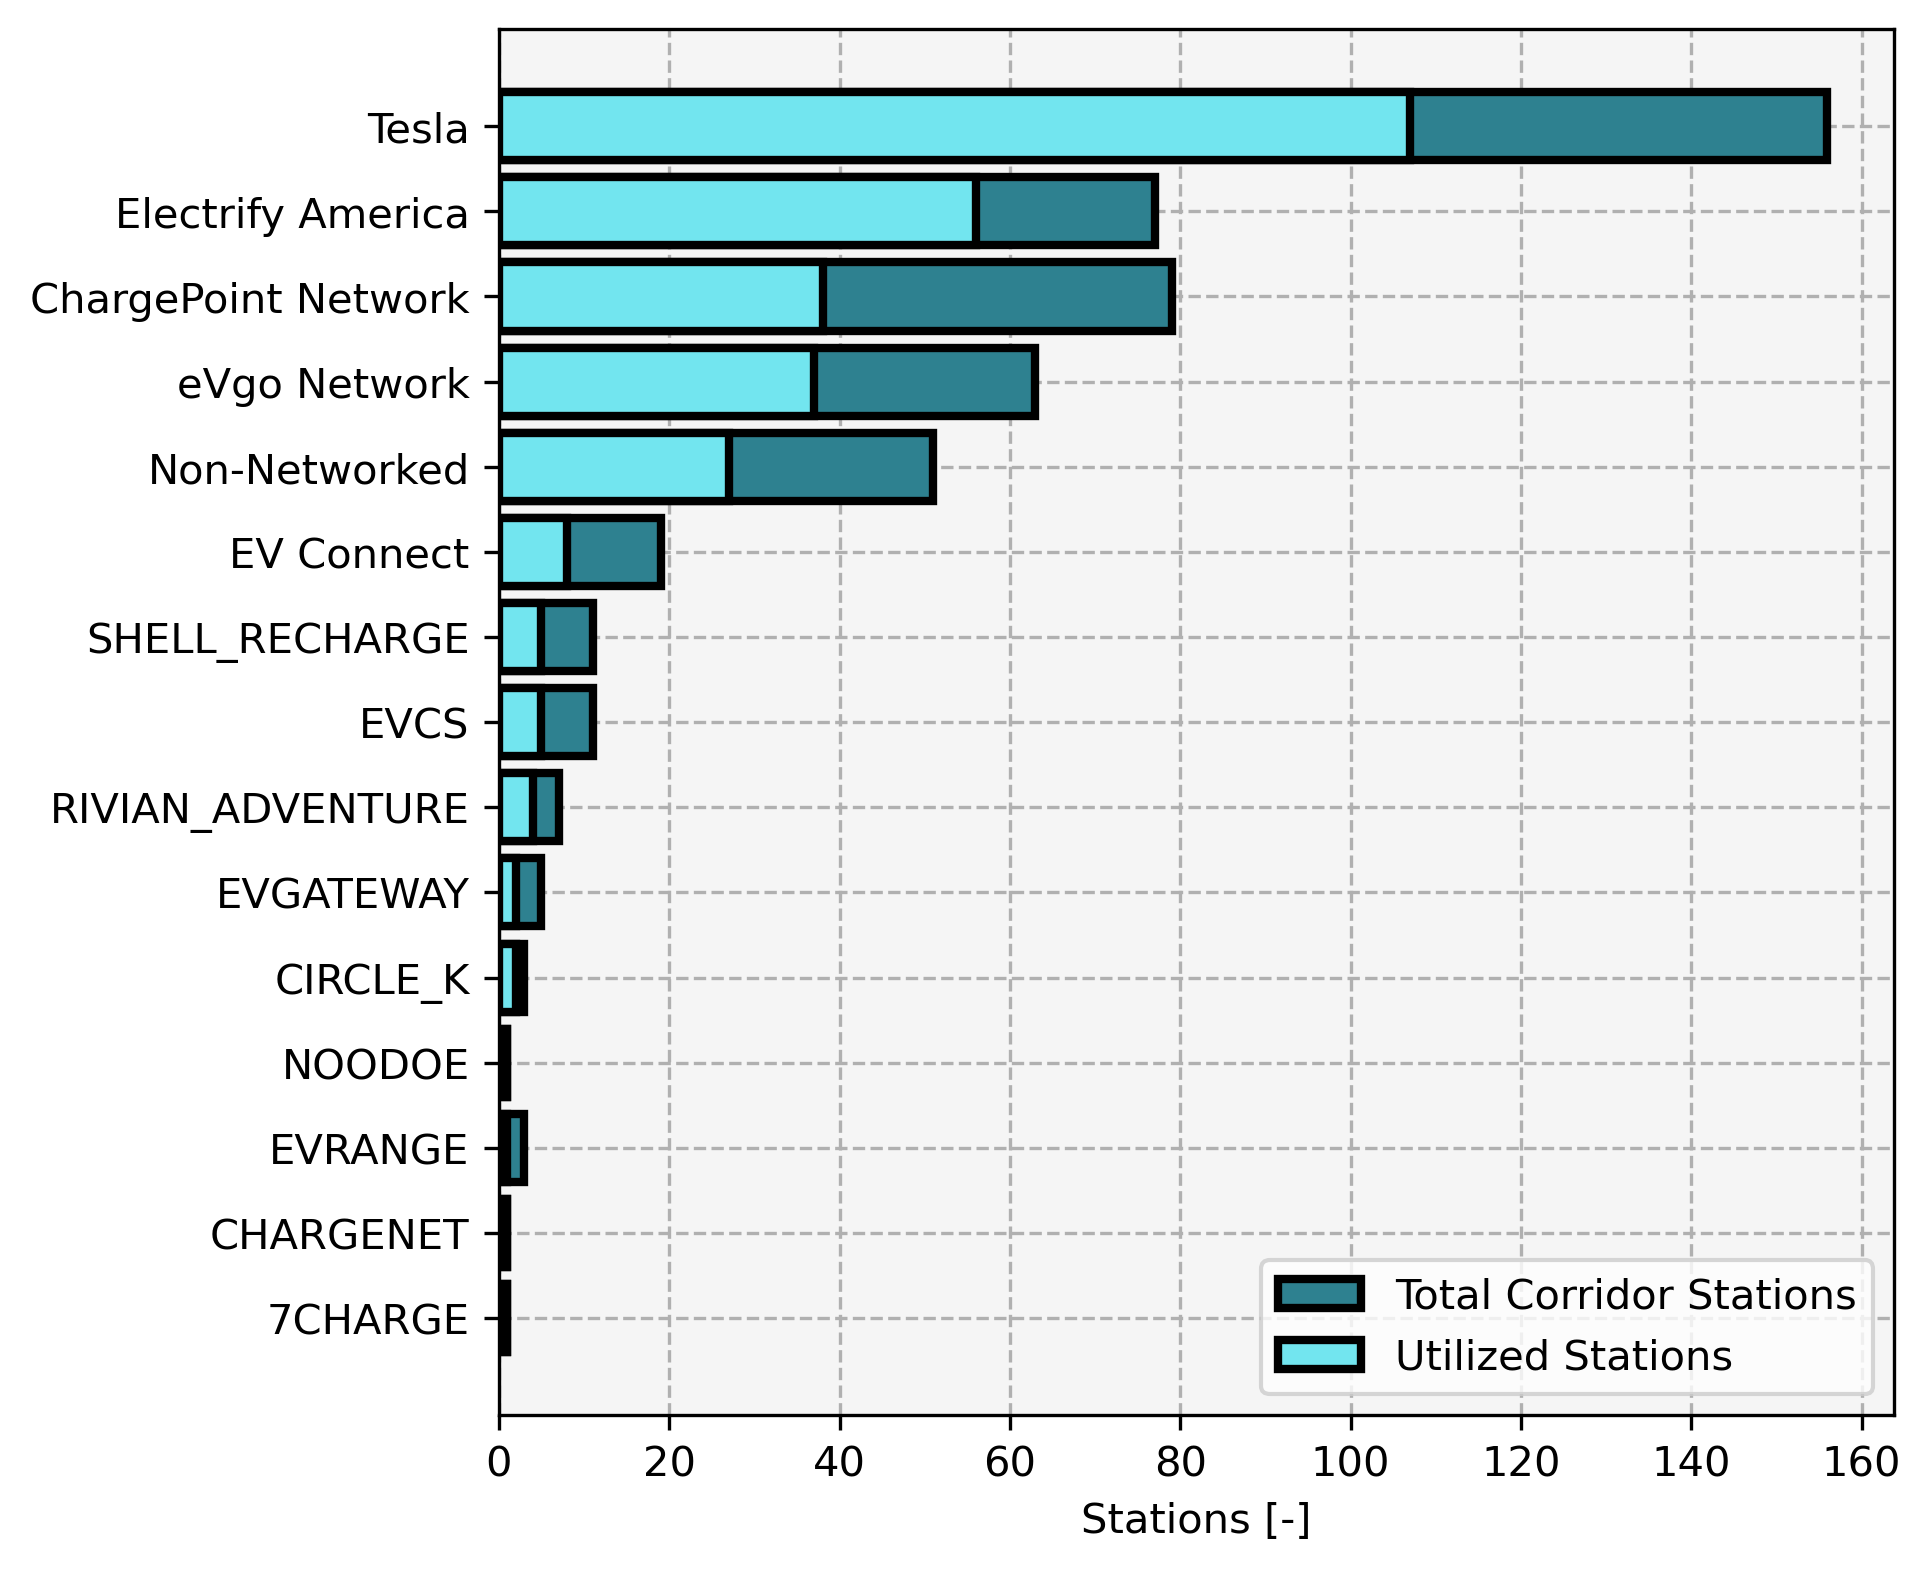
\includegraphics[width = \linewidth]{figs/corridor_station_utilization.png}
	\caption{Corridor DC charging network utilization rates}
	\label{fig:utilization_rates}
\end{figure}

\begin{figure}[H]
	\centering
	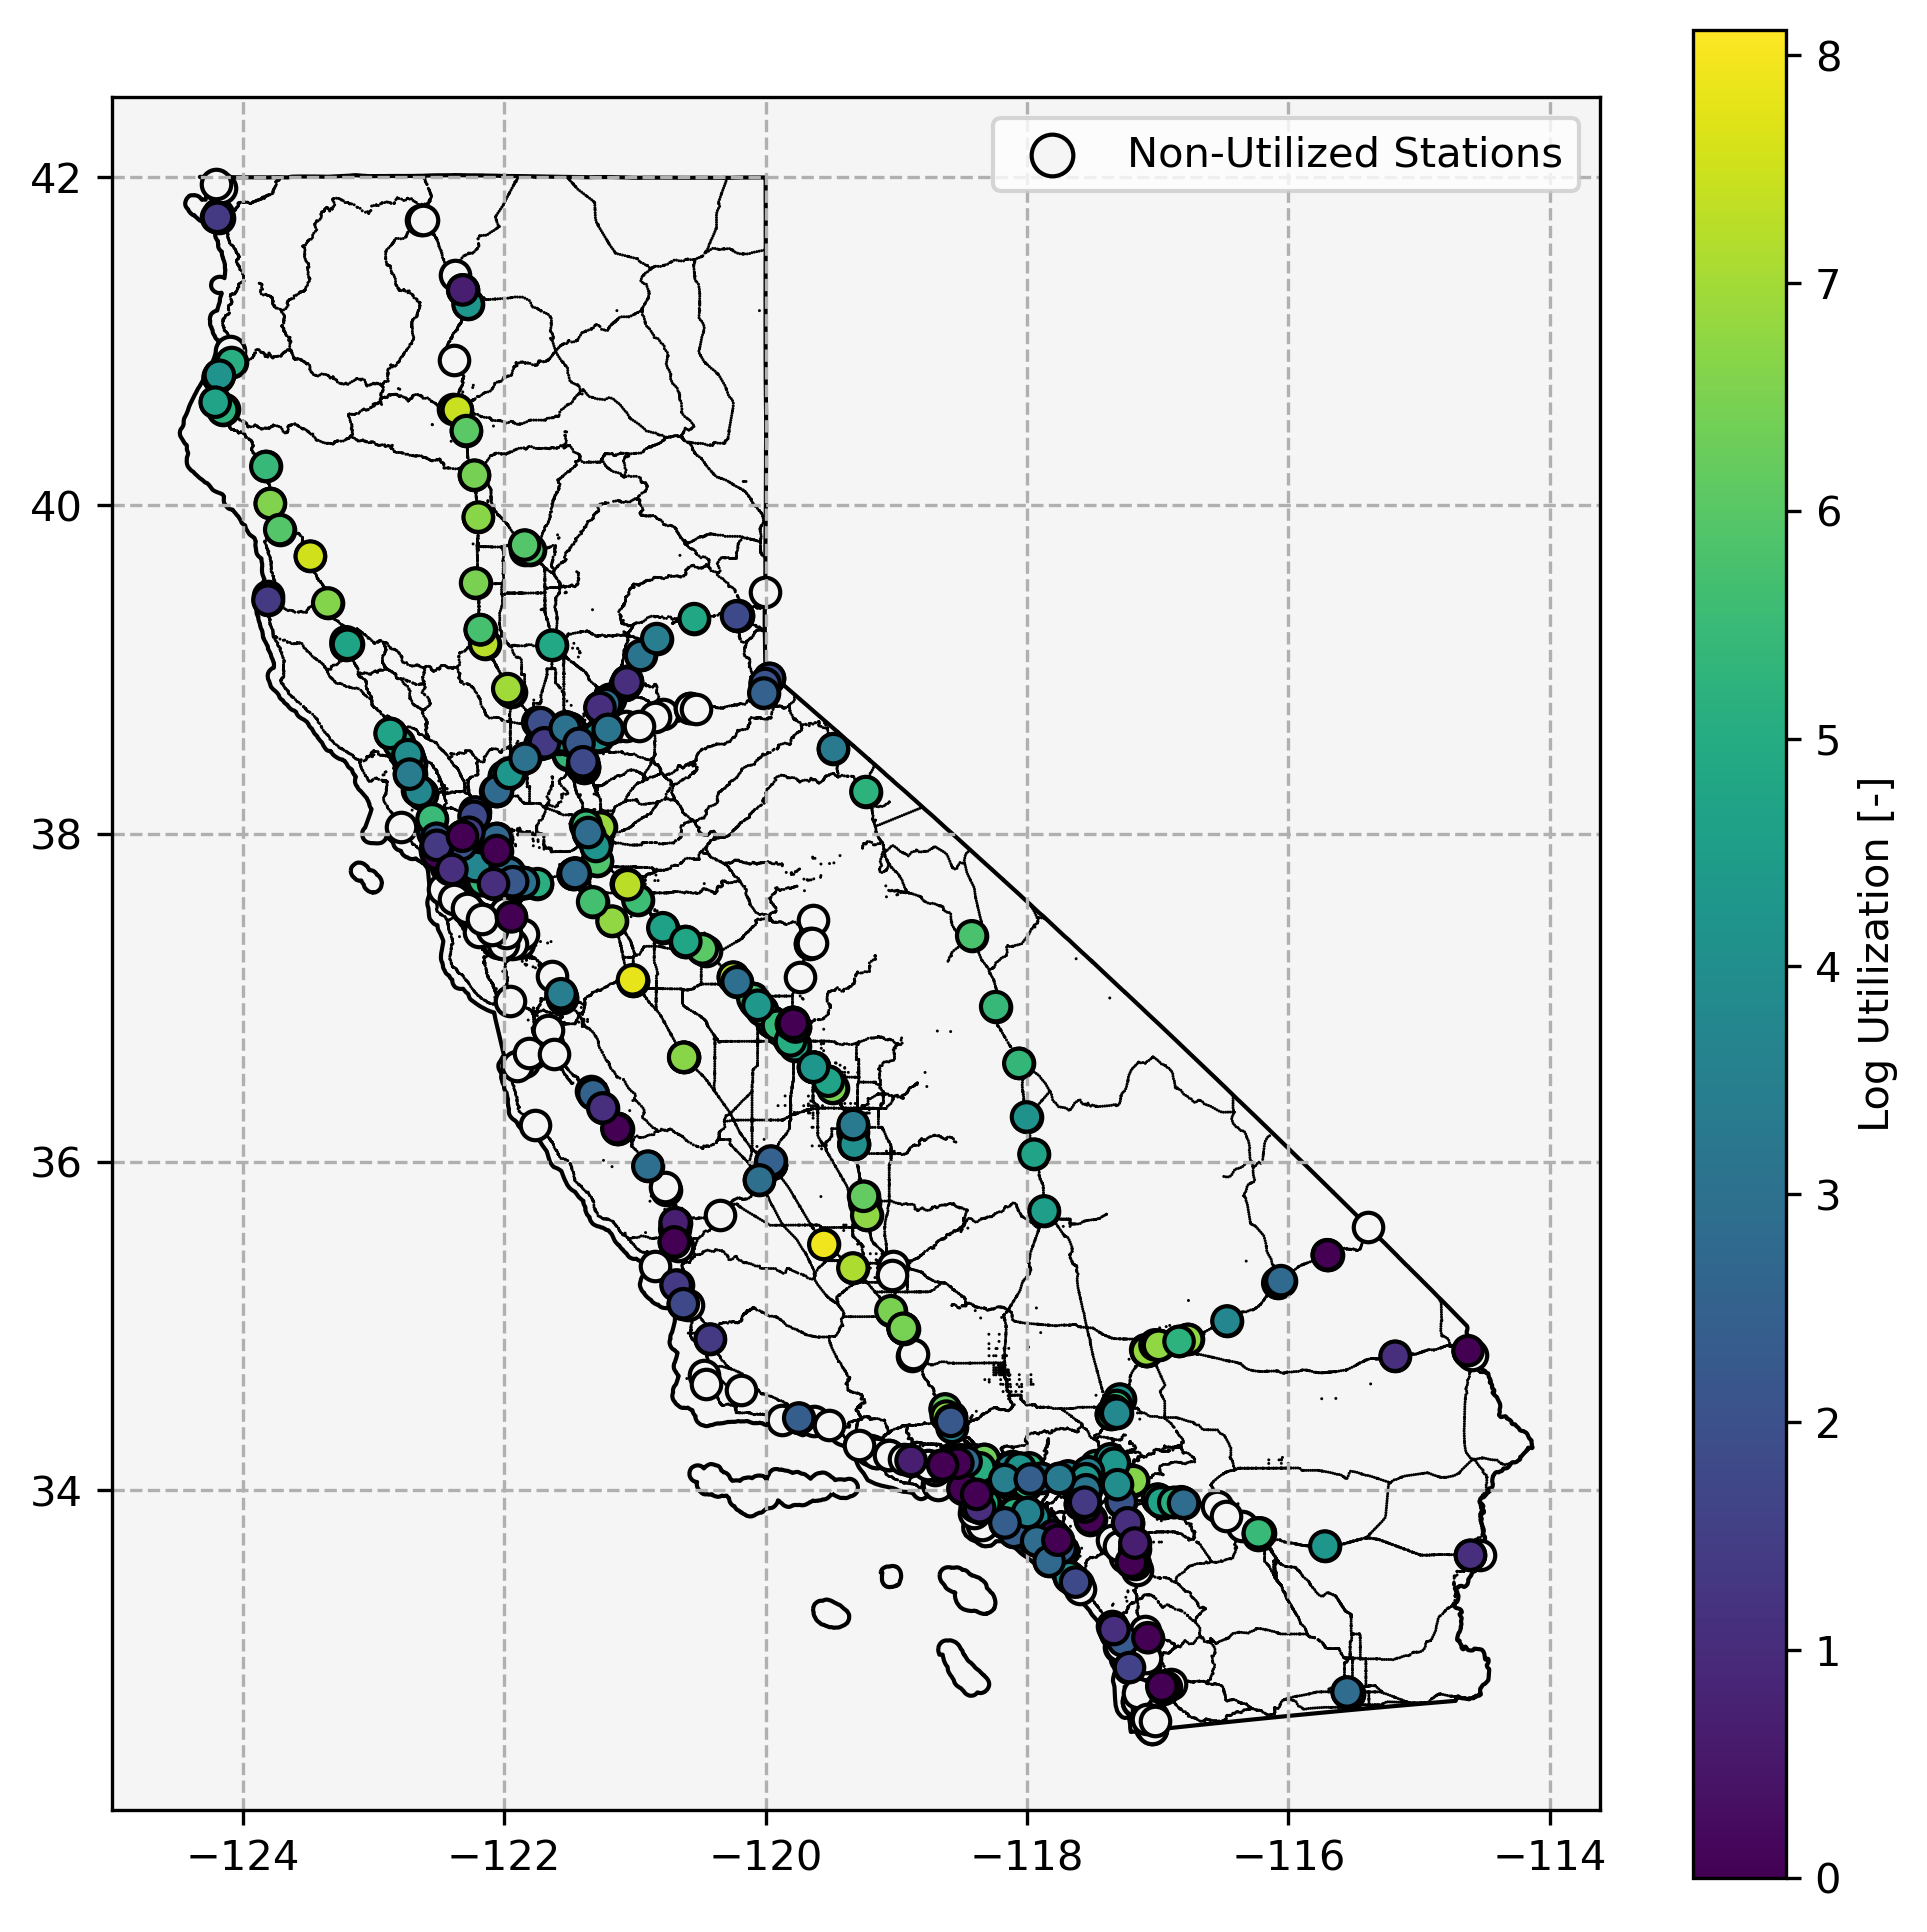
\includegraphics[width = \linewidth]{figs/California_SNG_Utilization.png}
	\caption{Corridor DC charging station log utilization}
	\label{fig:utilized_stations}
\end{figure}

It follows intuition that those chargers most useful for drivers are those located between cities on busy transportation corridors and this is backed up in this study. It also follows intuition that those chargers most likely to see use are those with higher redundancy in-station and lower redundancy in-corridor. In this sense Tesla stations are well positioned to absorb traffic should they become fully open to the general light duty \gls{ev} fleet. When one single entity has control over the locations of all stations in a network, that entity can concentrate chargers to maximize in-station redundancy and minimize between-station redundancy. That entity can, then strategically locate the highly concentrated stations. The result should be a network which experiences high utilization at each station and can benefit from economies of scale. When each network is developed by an independent actor these actors must build out their networks under the fear that a competitor could build a competing station near any of their stations at any time. The risk of building a large station only to lose business to a nearby competitor combined with the opportunity cost of not using limited capital to do the same inevitably results in a more inefficient combined network. However, many of the issues inherent with the distributed structure could be mitigated if the uncertainty and latency issues inherent to such a network could be mitigated. These issues can, possibly, be mitigated by an integrated status reporting and reservation system.


Often, the case for \glspl{bev} is made on an economic basis as \gls{bev} may have lower levelized costs of driving. This study focuses on travel times and routing did not optimize for cost. Partly, this is because at present there is no publicly available data on energy costs at a granular station-level for either gasoline or DC fast charging stations. Nevertheless, some sense of the relative economics of long-trip travel can be attained by examining energy costs per km. Energy costs vary substantially by region in the US with California being the most expensive. Energy costs around the time of writing are shown in Table \ref{tab:energy_costs}.

\begin{table}[H]
	\centering
	\caption{Residential electricity and petroleum average prices USD}
	\label{tab:energy_costs}
	\begin{tabular}{|C{.31\linewidth}|C{.23\linewidth}|C{.23\linewidth}|C{.23\linewidth}|}
		\hline Source & US & California & Percentage Increase \\
		\hline Petroleum [gallon] & 3.609 & 5.138 & 42.37 \\
		\hline Residential Electricity [kWh] & 0.1668 & 0.3247 & 94.66 \\
		\hline Transportation Electricity [kWh] & 0.1520 & 0.1191 & 27.62 \\
		\hline DC Fast Charging (Estimated) [kWh] & 0.35 - 0.50 & 0.35 - 0.60 & 0 - 20 \\
		\hline
	\end{tabular}
\end{table}

Petroleum prices are from AAA \cite{AAA_2024} and electricity prices are from EIA \cite{EIA_2024}. DC fast charging pricing schemes display much heterogeneity and may not be as easily accounted as metered electricity prices. An Ad-Hoc Text Mining study performed on over 90,000 recorded PlugShare events from 2019 and 2021 found the mode of DC fast charging prices to be in the range of 0.3 and 0.4 USD per kWh \cite{Trinko_2021}. Prices did not significantly correlate with local energy prices. In the same time period California residential electricity increased from 0.1995 USD per kWh to 0.2282 USD per kWh and transportation electricity increased from 0.0891 to 0.1179 USD per kWh. By comparison with 2024 electricity prices, one would expect prices in the range of 0.35 and 0.60 USD per kWh for DC fast charging in California and 0.35 to 0.5 in the US, ranges backed by informal reporting \cite{CalTrans_2024, Sowder_2024}. Thus, expected energy costs per highway km traveled can be computed and are shown in Table \ref{tab:expected_energy_costs_per_km}.

\begin{table}[H]
	\centering
	\caption{Expected energy costs per highway km traveled in US cents.}
	\label{tab:expected_energy_costs_per_km}
	\begin{tabular}{|C{\linewidth / 4}|C{\linewidth / 4}|C{\linewidth / 4}|C{\linewidth / 4}|}
		\hline Vehicle & Source & US Price & CA Price \\
		\hline Prius & Petroleum & 4.00 & 5.70 \\
		\hline Golf & Petroleum & 5.47 & 7.78 \\
		\hline Pacifica & Petroleum & 8.97 & 12.77 \\
		\hline \gls{bev} & Residential Electricity & 2.82 & 5.48 \\
		\hline \gls{bev} & DC Fast Charging & 5.91 - 8.44 & 5.91 - 10.13 \\
		\hline
	\end{tabular}
\end{table}

In the US, DC fast charging a \gls{bev} presents no appreciable economic benefit over fueling an efficient \gls{icev}. In much of the US, home-charging a \gls{bev} provides cost savings for daily travel and the initial part of a long trip. This is not the case in California where residential electricity is, on average, nearly twice as expensive as in the US as a whole.

If \glspl{bev} are a worse option than efficient \glspl{icev} for long trips on a time basis and no better on an energy cost basis this will make them less appealing to customers who value the ability to make long road trips. That customers seem to so highly value these uncommon events is a continuing source of frustration for \gls{bev} advocates. Negative perceptions of \gls{bev} long trip utility on consumer stated preference were found to be quite important in the late 2010s \cite{Skippon_2016, Hardman_2016, Franke_2017, Schmalfuss_2017}. In the intervening time period \gls{bev} ranges and maximum charge rates have markedly increased. Nevertheless, negative perceptions related to long trip utility persist for purchasers \cite{Bhat_2022, Paradies_2023, Corradi_2023, Philip_2023} and \gls{bev} range is a significant factor in determining usage share of \glspl{bev} in multi-vehicle household fleets \cite{Chakraborty_2022}. In the same time period, a massive build-out of DC charging infrastructure has taken place yet is not evident that the increased presence of DC charging infrastructure changes perceptions \cite{Hoogland_2023}.

As shown in Figure \ref{fig:utility_factors}, a \gls{bev} with 300 km of range can accomplish 80\% of US daily itineraries on a single charge. Fundamentally, the reality is that home or work charging leads to operational costs that often cheaper and rarely more expensive than petroleum. Similarly, home and work charging can lead to convenience benefits for \glspl{bev} as compared to \glspl{icev} \cite{Rabinowitz_2023} as \glspl{icev} require trips and trip deviations to reach supply stations. In theory, the trade-off of lower cost routine travel for higher cost long-distance travel is one which works in favor of \glspl{bev}. This is the logic which underpins the "charging pyramid" model which places long dwell charging events at its base and corridor DC fast charging events at the top. This model is also, to some degree, self-reinforcing. Because \gls{bev} drivers prefer AC charging, DC charging infrastructure has limited revenue potential leading to lower network capacity. Lower network capacity, in turn, leads to the perception that the network is inadequate and should be avoided.

The charging pyramid implies a different way of thinking about the role of car travel as a subset an individual's travel needs. Personal travel is inherently multi-modal and, for many \gls{od} arcs and many individuals, the cost differential between different modes is within the threshold of disambiguation. The strengths and weaknesses of \glspl{bev} as compared to \glspl{icev} may shift more short trips away from local transit and towards cars while shifting more long trips away from cars to air travel and inter-city transit. \glspl{bev} will only be one part of future mobility, unable to meet transportation needs or environmental goals on their own. Investments in \gls{bev} corridor infrastructure should be considered alongside investments into other low carbon inter-city transit modes.